\documentclass[aps,pra, twocolumn]{revtex4-1}
\usepackage{amssymb,amsthm,amsmath,enumerate,url, natbib, graphicx, float, csvsimple, todonotes, enumitem}

\def\FCW{1.0\columnwidth}

\newcommand{\multi}[1]{\vec{#1}}
\newcommand{\bs}[1]{\boldsymbol{#1}}
\newcommand{\pr}{\mathrm{Pr}}
\newcommand{\pdiff}[2]{\frac{\partial #1}{\partial #2}}
\renewcommand{\d}{\mathrm{d}}
\newcommand{\M}{\mathcal{M}}
\newcommand{\R}{\mathcal{R}}
\newcommand{\Tr}{\mathrm{Tr}}
\newcommand{\Lik}{\mathcal{L}}
\renewcommand{\P}{\mathcal{P}}
\newcommand{\stup}{\uparrow}
\newcommand{\stdown}{\downarrow}
\newcommand{\stleft}{\leftarrow}
\newcommand{\stright}{\rightarrow}
\newcommand{\styplus}{\nearrow}
\newcommand{\styminus}{\swarrow}
\newcommand{\reals}{\mathbb{R}}
\newcommand{\cH}{\mathcal{H}}
\newcommand{\cL}{\mathcal{L}}
\newcommand{\Id}{\mathbb{I}}
\newcommand{\cI}{\mathcal{I}}
\newcommand{\ket}[1]{\ensuremath{\left|#1\right\rangle}}
\newcommand{\bra}[1]{\ensuremath{\left\langle\scriptstyle#1\right|}}
\newcommand{\braket}[2]{\ensuremath{\left\langle\scriptstyle#1|#2\right\rangle}}
\newcommand{\ketbra}[2]{\ket{#1}\!\!\bra{#2}}
\newcommand{\expect}[1]{\ensuremath{\left\langle#1\right\rangle}}
\newcommand{\braopket}[3]{\ensuremath{\bra{#1}#2\ket{#3}}}
\newcommand{\proj}[1]{\ketbra{#1}{#1}}
\newcommand{\union}{\cup}
\def\Id{1\!\mathrm{l}}
\newcommand{\Fi}{\mathcal{I}}

\newcommand{\bvec}[1]{\boldsymbol{#1}}
 

\newcommand{\rhohat}{\hat{\rho}}
\newcommand{\rhoBME}{\rhohat_{\scriptscriptstyle\mathrm{BME}}}
\newcommand{\rhoML}[1]{\rhohat_{\scriptscriptstyle{\mathrm{ML},#1}}}
\newcommand{\rhotomo}{\rhohat_{\scriptscriptstyle\mathrm{tomo}}}
\newcommand{\rhotrue}{\rho_{\scriptscriptstyle\mathrm{true}}}
\newcommand{\phat}{\hat{p}}

\newcommand{\diff}{\mathrm{d}\!}
\newcommand{\diffk}[1]{\mathrm{d}_{#1}\!}

\begin{document}
\author{Travis L Scholten}
\author{Robin Blume-Kohout}
\affiliation{Center for Computing Research (CCR), Sandia National Labs}
\affiliation{Center for Quantum Information and Control (CQuIC), University of New Mexico}

\title{Behavior of the Maximum Likelihood in Quantum State Tomography}

\begin{abstract}
Quantum state tomography on a $d$-dimensional system demands resources -- for example, experimental repetitions, or data post-processing -- that grow rapidly with $d$. They may be reduced by using \emph{model selection} to tailor the number of parameters used to model the data.  Most model selection methods typically rely on a null theory for test statistics, describing their behavior when two models are equally good; we focus on the behavior of the \emph{loglikelihood ratio statistic}.  Because quantum tomographic models do not generally satisfy \emph{local asymptotic normality}, due to the positivity constraint $\rho\geq 0$, the classical null theory (the \emph{Wilks theorem}) should not be used.  Thus, understanding and quantifying how positivity constrains the null theory of test statistics is vital for enabling model selection in state tomography.  Here, we define a new generalization of local asymptotic normality, \emph{local asymptotic metric-projected normality}, show that quantum tomographic models satisfy it, and derive a replacement for the Wilks theorem. In addition to enabling reliable model selection, our results shed more light on the qualitative effects of the positivity constraint on state tomography.
\end{abstract}
\date{\today}

\maketitle


Determining the quantum state $\rho_{0}$ produced by a specific preparation procedure for a quantum system is a problem almost as old as quantum mechanics itself. This task, known as \emph{quantum state tomography} \cite{Paris2004}, is not only useful in its own right (diagnosing and detecting errors in state preparation), but is also used in other characterization protocols including entanglement verification \cite{Steffen2006, Blume-Kohout2010c, VanEnk2007} and process tomography \cite{Anis2012}. A typical state tomography protocol proceeds as follows: many copies of $\rho_{0}$ are produced; they are measured in diverse ways; and finally the outcomes of those measurements (data) are collated and analyzed to produce an estimate $\rhohat$.  This is a straightforward statistical inference process \cite{Reid2015, Wasserman2004}, where the data are used to fit the parameters of a statistical model.  However, we don't always know what model to use.  In state tomography, the parameter is $\rho$, and the model is the set of all possible density matrices on a Hilbert space $\cH$ (equipped with the Born rule). It is not always \emph{a priori} obvious what $\cH$ or its dimension is; examples include optical modes \cite{Altepeter2005, Bertrand1987, Lvovsky2009, Breitenbach1997, Leonhardt1995} and leakage levels in AMO and superconducting \cite{Motzoi2009, Fazio1999} qubits. In such situations, we seek to let the data itself determine which of many candidate Hilbert spaces is best suited for reconstructing $\rho_{0}$.

Choosing an appropriate Hilbert space on the fly is an instance of a general statistical problem called \emph{model selection}.  Although model selection has been thoroughly explored in classical statistics \cite{Burnham2004}, its application to quantum tomography encounters some obstacles.  They stem from the fact that quantum states (and therefore, estimates of them) must satisfy a \emph{positivity constraint} ($\rho\geq0$).  A similar constraint (complete positivity) applies to process tomography.  The impact of positivity constraints on state and process tomography is an active area of research \cite{Candes2006, Flammia2012a, Suess2016, Carpentier2015}, and its implications for model selection have also been considered \cite{Schwarz2013a, Guta2012a, VanEnk2013a, Langford2013, Yin2011, Moroder2013, Knips2015}.  In this paper, we address a specific question at the heart of this matter:  \emph{How does the loglikelihood ratio statistic used in many model selection protocols, including (but not limited to) information criteria such as Akaike's AIC \cite{Akaike1974}, behave in the presence of the positivity constraint $\rho\geq0$}? 

We begin in Section \ref{sec:intro} by introducing $\lambda$, the loglikelihood ratio statistic, and outline how it can be used to choose a Hilbert space dimension.  In Section \ref{sec:qstmodelselection}, we show how and why the standard result for its behavior, the Wilks theorem, falls apart in the presence of the positivity constraint, because the constraint causes quantum state space to not satisfy \emph{local asymptotic normality} (LAN).  We define a new generalization of LAN, \emph{local asymptotic metric-projected normality}, in Section \ref{sec:lanreplacement}; this generalization explicitly accounts for the positivity constraint, and is satisfied by quantum state space. Using this generalization, we derive a closed-form approximation for $\lambda$'s expected value in Section \ref{sec:computingllrs}, thereby providing a replacement for the Wilks theorem that \emph{is} applicable in state tomography.  Finally, we test the validity of our approximate theory under the assumptions used in its derivation (Section \ref{sec:theorycomp1}), and under harsh conditions by comparing it to numerical results for the realistic problem of optical heterodyne tomography (Section \ref{sec:heterotomo}).

\section{Introduction - Statistical Model Selection}
\label{sec:intro}
Discussing model selection for state tomography requires introducing some basic statistical notions.  A \emph{model} is a parameterized family of probability distributions over some data $D$, usually denoted as $\mathrm{Pr}_{\bs{\theta}}(D)$, where $\bs{\theta}$ are the \emph{parameters} in the model. In quantum state tomography, the data are the outcomes of the measurements of a positive operator-valued measure (POVM) $\{E_{j}\}$, the parameters are a quantum state $\rho$, and the probability of observing outcome ``$j$" is given by the Born rule: $p_{j} = \mathrm{Tr}(\rho E_{j})$ \footnote{The index $j$ may be continuous or discrete.}. In this paper, a model is a set of density matrices, and a state $\rho$ is a particular choice of the model's parameters.

Suppose we have some data obtained from an unknown state $\rho_{0}$, and two candidate models $\M_{1}, \M_{2}$ that could be used to fit it.  Many of the known methods for choosing between them (i.e., model selection) involve quantifying how well each model fits the data by its \emph{likelihood}.  The likelihood of a simple hypothesis $\rho$ is defined as $\mathcal{L}(\rho) = \mathrm{Pr}(\mathrm{Data}|\rho)$.  Models, however, are \emph{composite} hypotheses, comprising many possible values of $\rho$.  A canonical way to define model $\M$'s likelihood is via the general method of \emph{maximum likelihood} (ML), by maximizing $\cL(\rho)$ over $\rho\in\M$.  In practice, the maximization is usually done explicitly to find an ML estimate $\hat{\rho}_{\mathrm{ML},\M}$ \cite{Hradil1997, JamesPRA2001, Blume-Kohout2010} of $\M$'s parameters, and then $\cL(\M) = \cL(\hat{\rho}_{\mathrm{ML},\M})$.  (Note: although it is common to refer to $\hat\rho_{\mathrm{ML}}$ without specifying the model over which $\cL$ was maximized, we list the model explicitly in the subscript because in this paper we are constantly maximizing over different models!)

Then, the models can be compared using the \emph{loglikelihood ratio} \cite{Neyman1933, Blume-Kohout2010, Moroder2013}:
\begin{align}
\lambda(\M_{1}, \M_{2}) &\equiv -2 \log \left(\frac{\cL(\M_{1})}{\cL(\M_{2})}\right)\\
&= -2 \log \left(\frac{\cL(\rhoML{\M_{1}})}{\cL(\rhoML{\M_{2}})}\right)\\
&= -2 \log \left(\frac{\underset{\rho \in \M_{1}}{\max}~\cL(\rho)}{\underset{\rho \in \M_{2}}{\max}~\cL(\rho)}\right).
\end{align}
All else being equal, a positive $\lambda$ favors $\M_2$ -- i.e., the model with the higher likelihood is more plausible, because it fits the data better.  However, all else is rarely equal.  If both models are equally valid -- e.g. they both contain $\rho_0$ -- but $\M_2$ has more parameters, then $\M_2$ will very probably fit the data better.  Models with more adjustable parameters do a better job of fitting \emph{noise} (e.g. finite sample fluctuations) in the data.  This becomes strictly true when the models are \emph{nested}, so that $\M_{1} \subset \M_{2}$.  In this case, the likelihood of $\M_{2}$ is at least as high as that of $\M_{1}$;  not only is $\lambda \geq 0$, but almost surely $\lambda > 0$.

Remarkably, the same effect also makes $\M_{2}$'s fit less accurate (almost surely), because that fit incorporates more of the noise in the data.  These two effects constitute \emph{overfitting}, which can be summed up as ``Extra parameters make the fit look better, but perform worse.''  An overfitted model would fit \emph{past/current} data extremely well,  but would fail to accurately predict \emph{future} data well. This provides strong motivation to correct for overfitting by penalizing or handicapping larger models, to prevent them from being chosen over smaller models that are no less valid, and may even yield better estimates in practice \cite{Akaike1974}.

For this reason, any model selection method that relies (explicitly or implicitly) on a statistic to quantify ``how well model $\M$ fits the data'' also relies on a \emph{null theory} to predict how that statistic will behave if $\rho_{0} \in \M$.  A model selection criterion based on an invalid null theory (or a criterion used in a context where its null theory does not apply) will tend to choose the wrong model.

The null theory may be used to formulate a \emph{decision rule} for choosing between two models. If we know how the statistic behaves when both models are equally good, then we can compare the observed value of the statistic to the null theory. If the observed value is very improbable under the null theory, then that constitutes evidence against the smaller model, and justifies rejecting it. On the other hand, if the observed value is \emph{consistent} with the null theory, there is no reason to reject the smaller model.

The standard null theory for $\lambda$ is the \emph{Wilks theorem} \cite{Wilks1938}. It relies on \emph{local asymptotic normality} (LAN) \cite{LeCam1970, LeCam1956}. LAN means that:
\begin{itemize}[nosep]
\item[(1)] As $N_{\mathrm{samples}}\rightarrow \infty$,  $\rhoML{\M}$ is normally distributed around $\rho_{0}$ with covariance matrix $\Fi^{-1}$:
\begin{equation}
\label{eq:landist}
\mathrm{Pr}(\rhoML{\M}) \propto \exp\left[-\mathrm{Tr}[(\rho_{0} - \rhoML{\M})\mathcal{I}(\rho_{0} -\rhoML{\M})]/2\right]
\end{equation}
\item[(2)]The likelihood function in a neighborhood of $\rhoML{\M}$ is locally Gaussian with Hessian $\Fi$:
\begin{equation}
\label{eq:lanl}
\mathcal{L}(\rho) \propto \exp\left[-\mathrm{Tr}[(\rho - \rhoML{\M})\mathcal{I}(\rho - \rhoML{\M})]/2\right]
\end{equation}
\end{itemize}
Here, $\Fi$ is the (classical) \emph{Fisher information matrix} associated with the POVM. It quantifies how much information the data carry about a parameter in the model.  (Note that in expressions involving $\mathcal{I}$, states $\rho$ are treated as vectors in state space, and $\mathcal{I}$ is a matrix or 2-index tensor acting on that state space). Generally speaking, the Fisher information depends strongly on $\rho_{0}$ and the POVM being measured. However, as the next section explains, it's common in classical statistics to assume \emph{regularity conditions} that make it possible to change to \emph{Fisher-adjusted} coordinates in which $\mathcal{I}$ is isotropic (i.e., $\mathcal{I} \propto \Id$).

Most statistical models satisfy LAN.  When LAN holds \emph{and} $N_{\mathrm{samples}}$ is large enough to reach the ``asymptotic" regime, the Wilks theorem states that, under suitable regularity conditions, if $\rho_{0}\in \M_{1}\subset \M_{2}$, where $\M_{2}$ has $K$ more parameters than $\M_{1}$, then $\lambda$ is a $\chi^{2}_{K}$ random variable.  This is a complete null theory for $\lambda$ (under the specified conditions), and implies that $\langle \lambda \rangle = K$ and $(\Delta \lambda)^{2} = 2K$.

Therefore, in the ``Wilks regime", a simple rule for model selection would be to compare the observed value of $\lambda$ to $\lambda_{\mathrm{thresh}} = \langle \lambda \rangle + n\Delta \lambda$, for some $n \approx 1$, and reject the smaller model if $\lambda > \lambda_{\mathrm{thresh}}$.  While model selection rules can be more subtle and complex than this \cite{Akaike1974, Schwarz1978, Kass1995, Spiegelhalter2002}, they usually take the general form of a threshold in which $\expect{\lambda}$ plays a key role.  Rather than attempting to define a specific rule, our focus in this paper is to understand the behavior of $\expect{\lambda}$ and derive an approximate expression for it in the context of state tomography.

The first step in doing so is to explain how, and why, the Wilks theorem can break down for state tomography.

\section{Quantum State Tomography and The Breakdown of the Wilks Theorem}
\label{sec:qstmodelselection}
Quantum state tomography typically begins with $N$ independently and identically prepared quantum systems -- i.e., $N$ copies of an unknown state $\rho_{0}$.  Each copy is measured, and without loss of generality we can assume that each measurement is described by the same positive operator-valued measure (POVM).  A POVM is a collection of positive operators $\{E_j\}$ summing to $\Id$, and the probability of outcome ``$j$'' is given by $\Tr(\rho_0 E_j)$.  The results of all $N$ measurements constitute data, represented as a record of the frequencies of the possible outcomes $\{n_{j}\}$, where $n_{j}$ is the number of times ``$j$'' was observed, and $\sum_{j}n_{j} = N$.  Finally, this data is processed through some \emph{estimator} to yield an estimate of $\rho_0$, denoted $\hat{\rho}$ .  A variety of estimators have been proposed \cite{Vogel1989,Hradil1997,JamesPRA2001,Blume-Kohout2010b,Blume-Kohout2010,Zhu2014a,Ferrie2016}, but they are not our concern here.  However, since we \emph{are} concerned with computing the likelihood of a model $\M$, which is defined as the likelihood of the most likely $\rho\in\M$, we will make extensive use of the \emph{maximum likelihood} (ML) estimator $\rhoML{\M}$.  This should not be taken as advocacy for the ML estimate; it is only a convenient way to find the maximum of $\cL$ over $\M$ as $\mathcal{L}(\rhoML{\M})$, and once a model is chosen, a different estimator could be used.

The likelihood $\mathcal{L}(\rho)$ is
\begin{equation}
\mathcal{L}(\rho) = \prod_{j}\mathrm{Tr}(\rho E_{j})^{n_{j}},
\end{equation}
so $\rhoML{\M}$ is the solution to the optimization problem
\begin{equation}
\label{eq:mle}
\rhoML{\M} = \underset{\rho \in \M}{\text{argmax}}~\mathcal{L}(\rho) = \underset{\rho \in \M}{\text{argmin}}~-\log(\mathcal{L}(\rho)).
\end{equation}
In state tomography, $\M$ is almost always the set of all density matrices over a Hilbert space $\cH$:
\begin{equation}
\mathcal{M}_{\cH} = \{\rho~|~\rho \in \mathcal{B}(\mathcal{H}),~\mathrm{Tr}(\rho) =1,~\rho \geq 0\},
\end{equation}
where $\mathcal{B}(\cH)$ is the space of bounded linear operators on $\cH$.  To solve the optimization problem, we can use the following facts: (a) $\M_{\cH}$ is a convex set, and (b) $\rhoML{\M}$ minimizes the value of $-\log(\cL(\rho))$, which is a convex function. Thus, because $\rhoML{\M}$ is the solution to minimizing a convex function defined over a convex set, it can be found efficiently via any of several algorithms for convex optimization \cite{Boyd}.

Usually, $\cH$ is taken for granted or chosen by fiat.  In this paper, we will consider a nested family of different Hilbert spaces, indexed by their dimension $d$: $\cH_{1}  \subset \cdots \subset \cH_{d} \subset \cH_{d+1} \subset \cdots$.  The models we consider are therefore given by:
\begin{equation}
\label{eq:modelsd}
\M_{d} \equiv \mathcal{M}_{\cH_{d}} = \{\rho~|~\rho \in \mathcal{B}(\mathcal{H}_{d}),~\mathrm{Tr}(\rho) =1,~\rho \geq 0\}.
\end{equation}
For notational brevity, we will use $\rhoML{d}$ to denote the ML estimate in $\M_{d}$. To select between these models, we need to determine whether one model (say, $\M_{d + 1}$) is ``better'' than another (say, $\M_{d}$).  To evaluate which is better, we typically compute the likelihood of each model, and then use $\lambda(\M_{d}, \M_{d+1})$ to choose between them. As mentioned in the previous section, this requires having a \emph{null theory} for $\lambda$ that describes its behavior when both models are valid, i.e. when $\rho_{0} \in \M_{d},\M_{d + 1}$.

The Wilks theorem, which is the classical null theory for $\lambda$, relies on local asymptotic normality (LAN). In classical statistics, it is common to assume that boundaries are not relevant, either because the models of interest have none, or by assuming that the true parameter values $\rho_{0}$ lie far away from them.  In the absence of boundaries, and in the asymptotic limit where curvature of the Fisher metric is also negligible, many statistics calculations can be simplified by changing to \emph{Fisher-adjusted} coordinates in which the Fisher information is isotropic (i.e., $\mathcal{I}\propto\Id$). It is these two properties of the models being compared -- that they satisfy LAN, and their boundaries are either non-existent or sufficiently far away -- which enable the derivation of the Wilks theorem.

However, the statistical models used for quantum state tomography \emph{do} have boundaries. Given a model $\M_{d}$, we use the word ``boundaries" to denote the set of rank-deficient states within it. When $\rho_{0}\in \M_{d}$ and has rank $r = d$, LAN will hold -- which is to say that, asymptotically, the boundary can indeed be ignored. But when $\rho_{0}$ has rank $r<d$, it lies \emph{on} the boundary of the model (see Figure \ref{fig:boundaries}).  LAN does not hold, even in the asymptotic limit, because positivity constrains $\rhoML{d}$, and so $\mathrm{Pr}(\rhoML{d})$ is not Gaussian.  The Wilks theorem does not apply in this case.  (See Figure \ref{fig:boundaries2}.) Moreover, this is the relevant situation for our analysis, because \emph{even if $\rho_{0}$ is full-rank in $\M_{d}$, it must be rank-deficient in $\M_{d+1}$}.  So we require a replacement for the Wilks theorem, a null theory for $\lambda$ when $\rho_0$ is rank-deficient. 

\begin{figure}[h]
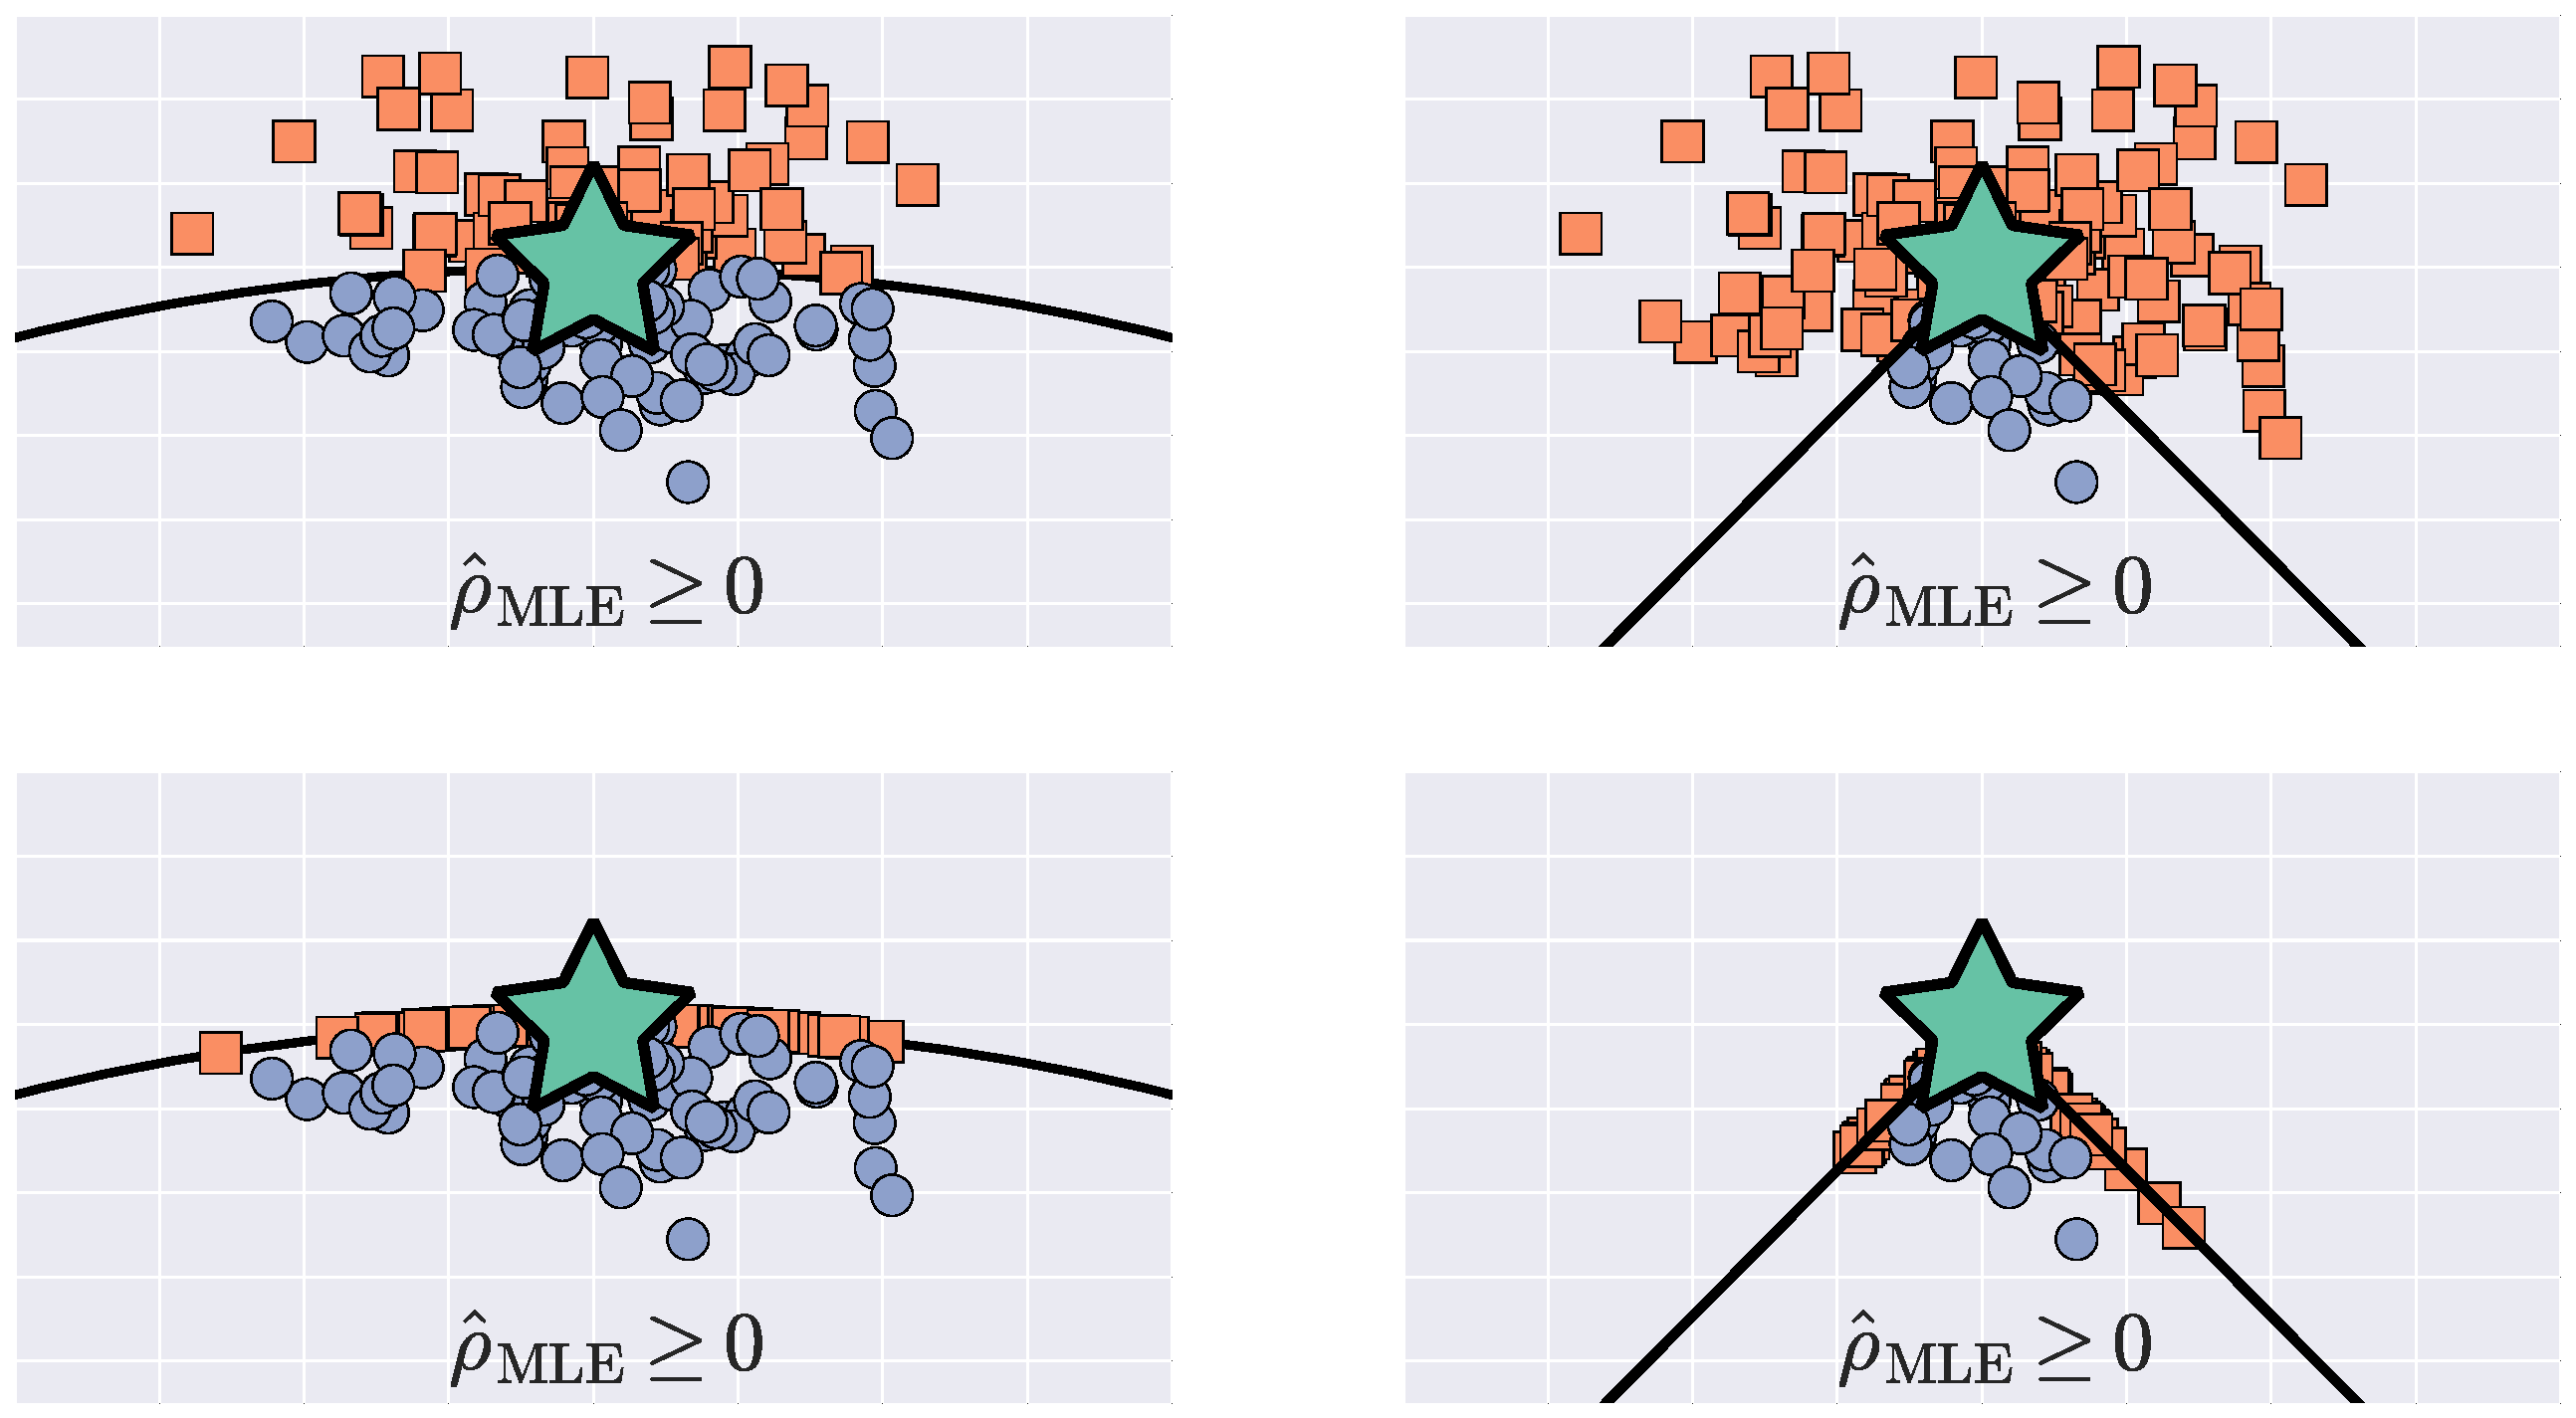
\includegraphics[width=\columnwidth]{Images/Figure_1.pdf}
 \caption{Two views of the impact of the boundary on maximum likelihood tomography of a qutrit state $\rho_{0}$ (star). \textbf{Top}: Without the positivity constraint, some estimates (orange squares) are not positive semidefinite; they do not represent valid estimates of a quantum state. However, some estimates (blue circles) are positive.
\textbf{Bottom}:  Imposing the positivity constraint causes the (previously unconstrained) estimates to ``pile up" on the boundary of state space, meaning that the \emph{local asymptotic normality} property doesn't hold, thereby invalidating the assumptions necessary to use the Wilks theorem in model selection.}
\label{fig:boundaries}
\end{figure}

\begin{figure}
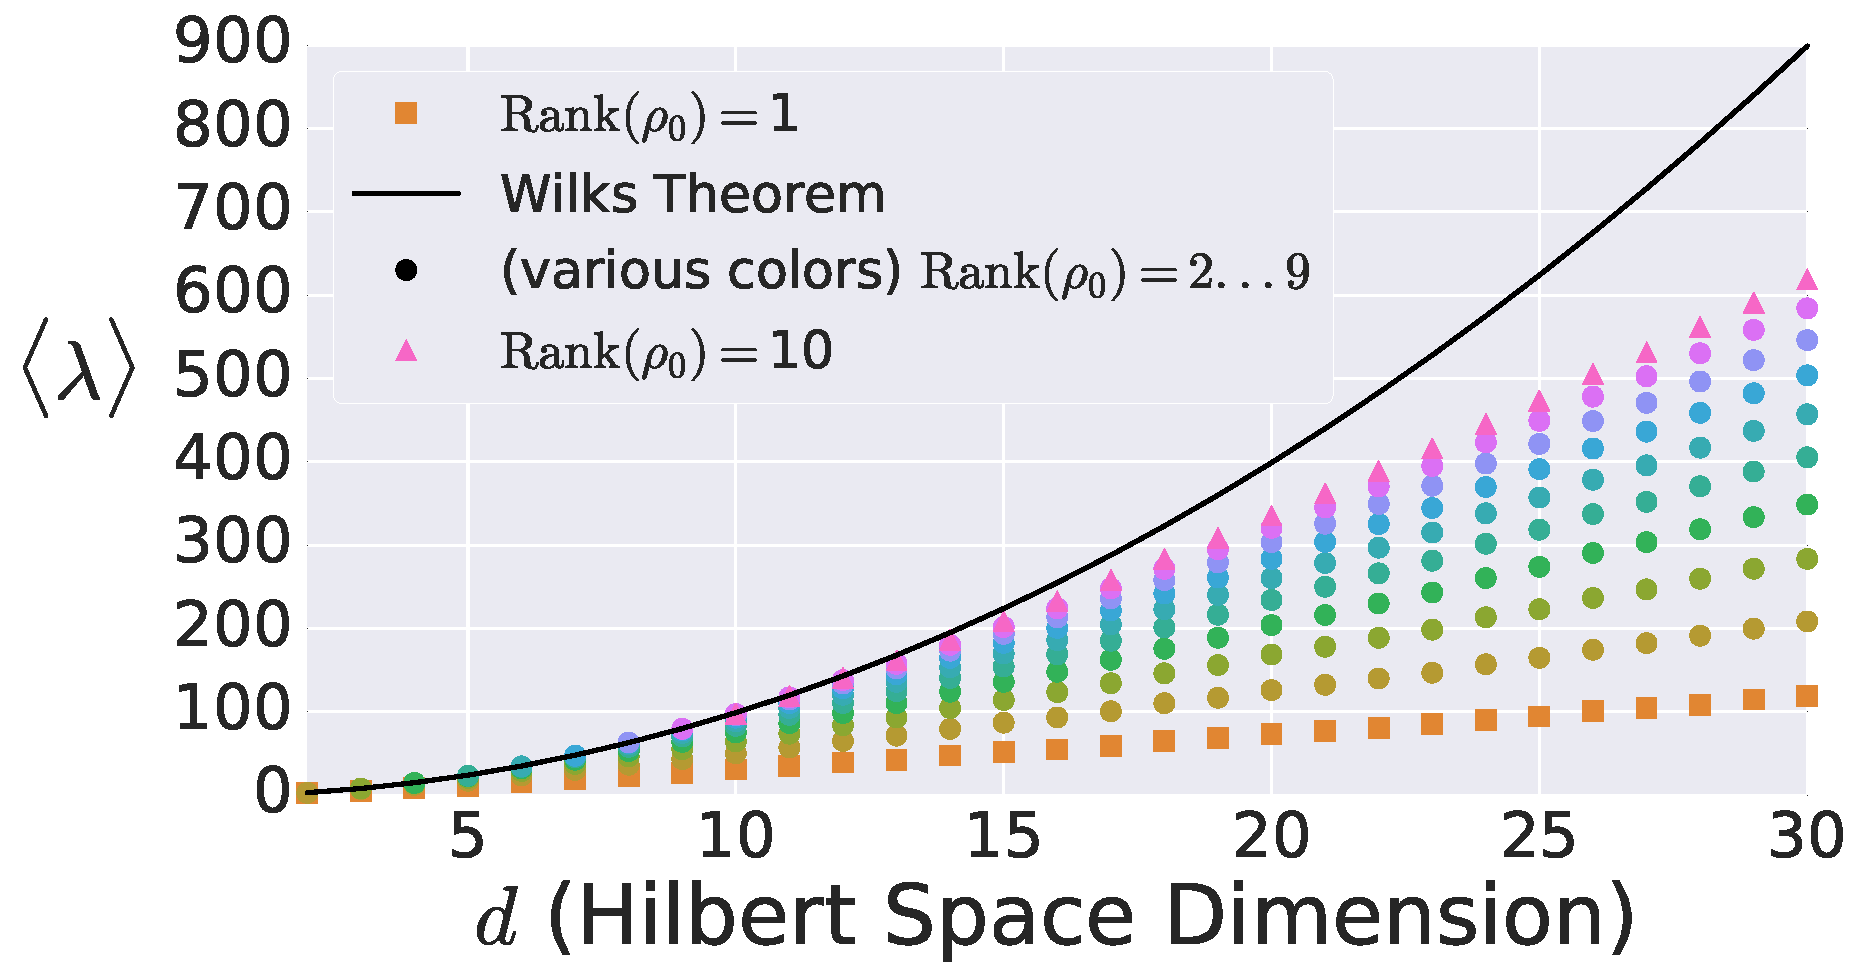
\includegraphics[width=\columnwidth]{Images/Figure_2A.pdf}
 \caption{Comparison of the classical theory (Wilks theorem) prediction for the loglikelihood ratio $\expect{\lambda}$ to numerical data for states $\rho_{0}$ with ranks $r=1,\ldots ,10$.  The Wilks theorem fails badly for low-rank states; our main result (Equation \ref{eq:ourLLRS}) gives a replacement that works correctly (see Figure \ref{fig:modelcomp-iso}).}
\label{fig:boundaries2}
\end{figure}

The next section of this paper is devoted to developing a framework for deriving a replacement for the Wilks theorem. This framework is a new generalization of LAN, called \emph{Local Asymptotic Metric-Projected Normality} (LAMPN). (For other generalizations of LAN, see \cite{Roussas2010, Jeganathan1982}.) Like LAN, LAMPN is a property that a statistical model may satisfy. Unlike LAN, LAMPN is satisfied for quantum tomographic models. For models which satisfy LAMPN, we compute an exact expression for $\lambda$, a necessary building block in our replacement for the Wilks theorem. In Section \ref{sec:computingllrs}, we show that the models $\M_{d}$ satisfy LAMPN, and derive an approximation for $\expect{\lambda}$; the main result is given in Equation \eqref{eq:ourLLRS}.  Section \ref{sec:theorycomparison} compares our theory to numerical results. Finally, Section \ref{sec:heterotomo} applies our theory to the problem of heterodyne tomography.

\section{Generalizing LAN to Deal with Constraints}
\label{sec:lanreplacement}

In this section, we define a framework that will allow us to derive a replacement for the Wilks theorem that is valid for rank-deficient $\rho_{0}$. To do so, we define a generalization of LAN in the presence of boundaries, which we call \emph{Local Asymptotic Metric-Projected Normality}.

\subsection{Definitions; Overview of Results}

The main definitions and results required for the remainder of the paper are presented in this subsection. Technical details and proofs are presented in the next subsection.

\textbf{Definition - Local Asymptotic Metric-Projected Normality (LAMPN)}: A statistical model $\M$ satisfies LAMPN if, and only if, $\M$ is a convex subset of a model $\M'$ which satisfies LAN.

Models which satisfy LAMPN have several nice properties:

\underline{First}: Asymptotically, the \emph{local state space} -- the region of $\M$ contained within a suitably-chosen ball centered at $\rho_{0}$ -- converges to the \emph{solid tangent cone} at $\rho_{0}$, denoted $T(\rho_{0})$.

\underline{Second}: $\rhoML{\M}$ is given by the \emph{metric projection} of $\rhoML{\M'}$ onto $T(\rho_{0})$:
\begin{equation}
\label{eq:lampnmle}
\rhoML{\M} = \underset{\sigma \in T(\rho_{0})}{\text{argmin}}~(\sigma  -\rhoML{\M'})\mathcal{I}(\sigma  -\rhoML{\M'}).
\end{equation}
(We first encountered the term ``metric projection" in the convex optimization literature \cite{McCoy2014, Amelunxen2014}, and it inspires our choice for the acronym ``LAMPN". However, it should be noted that in the problem setting considered in those references, $\mathcal{I} = \Id$.)

\underline{Third}: Asymptotically, the loglikelihood ratio $\lambda(\rho_{0}, \M)$, which is defined as
\[\lambda(\rho_{0}, \M) = -2 \log \left(\frac{\cL(\rho_{0})}{\underset{\rho \in \M}{\max}~\cL(\rho)}\right),\]
takes the following simple form
\begin{equation}
\label{eq:llrs_lan}
\lambda(\rho_{0}, \M) =  \mathrm{Tr}[(\rho_{0} - \rhoML{\M})\mathcal{I}(\rho_{0} - \rhoML{\M})].
\end{equation}
This property follows from the first and second properties, and is necessary for our derivation in Section \ref{sec:computingllrs} of $\langle \lambda \rangle$.

It should be noted that LAMPN is a property of $\M$ itself, not of the procedure we use to compute any estimate within it.. Further, its \emph{consequences} only hold asymptotically ($N_{\mathrm{samples}} \rightarrow \infty$). However, for sufficiently large $N_{\mathrm{samples}}$ such that we are in an ``asymptotic" regime, we can (and will!) use results derived in the asymptotic limit.

The following subsection presents the technical details and definitions to show the above results. The reader may skip it without loss of continuity, and proceed to Section \ref{sec:computingllrs}.

\subsection{Technical Details}

Consider a statistical model $\M$ which satisfies LAMPN. In the next sub-subsections, we prove the properties of $\M$ previously described.

\subsubsection{Convergence of the Local State Space to the Solid Tangent Cone}

In this sub-subsection, we show that, because the distribution of $\rhoML{\M'}$ is tightly concentrated around $\rho_{0}$ as $N_{\mathrm{samples}} \rightarrow \infty$, the behavior of $\rhoML{\M}$ is determined entirely within a shrinking ball around $\rho_{0}$. It turns out that, in the limit, the intersection of $\M$ and this ball is the \emph{solid tangent cone}.

Because $\M$ satisfies LAMPN, there exists a model $\M'$ of dimension $d'$ which satisfies LAN. This means as $N_{\mathrm{samples}} \rightarrow \infty$, the distribution of $\rhoML{\M'}$ satisfies
\[\mathrm{Pr}(\rhoML{\M'})\xrightarrow[]{\text{d}} \mathcal{N}(\rho_{0}, \Sigma/N_{\mathrm{samples}}),\]
where $\xrightarrow[]{\text{d}}$ means ``converges in distribution to", and $\Sigma = \mathcal{I}^{-1}$.
The shape of the distribution is entirely determined by $\mathcal{I}$. As $N_{\mathrm{samples}} \rightarrow \infty$, this Gaussian distribution becomes more and more tightly concentrated around $\rho_{0}$. There is still a non-zero probability that $\rhoML{\M'}$ will be arbitrarily far away from $\rho_{0}$. However, it is possible to find a ball $B$ of sufficient size such that it contains every $\rhoML{\M'}$ with probability 1 as $N_{\mathrm{samples}}\rightarrow \infty$.

Before doing so, we switch coordinates, by sending $\rho \rightarrow \rho - \rho_{0}$, thereby establishing $\rho_{0}$ as the origin of our coordinate system. In these coordinates, $\rhoML{\M'} \sim \mathcal{N}(0, \Sigma/N_{\mathrm{samples}})$, and we may easily prove the following lemma showing such a $B$ exists.

\textbf{Lemma}: Let $\rhoML{\M'} \sim \mathcal{N}(0, \Sigma/N_{\mathrm{samples}})$, and let $\lambda_{\max}(\Sigma)$ denote the largest eigenvalue of $\Sigma$. Define a ball $B = \{\rho \in \M' ~|~\mathrm{Tr}(\rho^{2}) \leq r^{2}\}$, where $r = \sqrt{\lambda_{\max}(\Sigma)}/N_{\mathrm{samples}}^{1/4}$. Then, $\lim_{N_{\mathrm{samples}} \rightarrow \infty} \mathrm{Pr}(\rhoML{\M'} \in B) =1$.

\textbf{Proof}: Let $B_{0}$ be an ellipsoidal ball defined by $\{\rho \in \M'~|~\mathrm{Tr}(\rho \Sigma^{-1} \rho) \leq r^{2}/N_{\mathrm{samples}}\}$, where $r^{2} = N^{1/2}_{\mathrm{samples}}$. Change coordinates by defining $\sigma = N_{\mathrm{samples}}^{1/2}\Sigma^{-1/2}\rho$. In these new coordinates
\[\hat{\sigma}_{\mathrm{ML},\M'} \sim \mathcal{N}(0, \Id_{d'}),~~~B_{0} = \{\sigma \in \M'~|~\mathrm{Tr}(\sigma^{2}) \leq r^{2}\},\]
and
\begin{align*}
\mathrm{Pr}(\hat{\sigma}_{\mathrm{ML},\M'} \in B_{0}) &= \mathrm{Pr}(\mathrm{Tr}(\hat{\sigma}_{\mathrm{ML},\M'}^{2}) \leq r^{2})\\
&= \int_{0}^{r^{2}}\chi^{2}_{d'}(z)~dz,
\end{align*}
because $\mathrm{Tr}(\hat{\sigma}_{\mathrm{ML},\M'}^{2})$ is a $\chi^{2}_{d'}$ random variable. From our choice of $r^{2}$, it follows that
\[\lim_{N_{\mathrm{samples}} \rightarrow \infty}~\mathrm{Pr}(\hat{\sigma}_{\mathrm{ML},\M'} \in B_{0})  =\int_{0}^{\infty}\chi^{2}_{d'}(z)~dz =1.\]
Switching back to the original coordinates, we have
\[B_{0} = \{\rho \in \M'~|~\mathrm{Tr}(\rho \Sigma^{-1} \rho) \leq 1/N_{\mathrm{samples}}^{1/2}\}.\]
Let's write the defining equation for $B_{0}$ in the standard quadratic form for an ellipsoid:
\[B_{0} = \{\rho \in \M'~|~\mathrm{Tr}(\rho ( N_{\mathrm{samples}}^{1/2}\Sigma^{-1} ) \rho) \leq 1\}.\]
The standard ellipsoid $\{\mathbf{x}~|~\mathbf{x}^{T}A\mathbf{x} \leq 1\}$ has semi-major axes whose lengths $s_{j}$ are related to the eigenvalues $a_{j}$ of $A$: $s_{j} = 1/\sqrt{a_{j}}$. The matrix $A = N_{\mathrm{samples}}^{1/2}\Sigma^{-1}$ has eigenvalues $N_{\mathrm{samples}}^{1/2}/\lambda_{j}$, where $\lambda_{j}$ are the eigenvalues of $\Sigma$. Thus, the lengths of the semi-major axes of $B_{0}$ are given by $s_{j} = 1/\sqrt{N_{\mathrm{samples}}^{1/2}/\lambda_{j}} = \sqrt{\lambda_{j}}/N_{\mathrm{samples}}^{1/4}$. Letting $\lambda_{\max}(\Sigma)$ denote the largest eigenvalue of $\Sigma$, the longest semi-major axis of $B_{0}$ has length $\sqrt{\lambda_{\max}(\Sigma)}/N_{\mathrm{samples}}^{1/4}$.
Because $B$ is a ball whose radius is equal to this length, $B_{0} \subset B$, and it follows that $\mathrm{Pr}(\rhoML{\M'} \in B_{0}) \leq \mathrm{Pr}(\rhoML{\M'} \in B)$. Because $\mathrm{Pr}(\rhoML{\M'} \in B_{0}) \leq \mathrm{Pr}(\rhoML{\M'} \in B) \leq 1$, and the asymptotic limit of $\mathrm{Pr}(\rhoML{\M'} \in B_{0})$ is 1, it follows from the squeeze theorem that $\lim_{N_{\mathrm{samples}\rightarrow \infty}}\mathrm{Pr}(\rhoML{\M'} \in B)=1$.
~\\~\\
Informally speaking, this lemma implies that ``all the action" about the MLEs $\rhoML{\M'}$ takes place inside $B$.

We now change coordinates so that, instead of have $B$ shrink,  $B, \M$, and $\M'$ all grow as $N_{\mathrm{samples}}$ increases. Consider the ``$N_{\mathrm{samples}}$-adjusted" coordinate system defined by $\sigma =  N^{1/4}_{\mathrm{samples}}\rho$. Notice the origin $(\rho_{0})$ remains unchanged, because of our earlier coordinate transformation that mapped it to 0. Under this transformation, $B$ is given by
\[B = \{\sigma \in \M'~|~\mathrm{Tr}(\sigma^{2}) \leq \sqrt{\lambda_{\max}(\Sigma)}N_{\mathrm{samples}}^{1/4}\}.\]
 The models $\M,\M'$ also expand under this transformation. However, they are not strict subsets of $B$ -- consider any $\rho \in \M, \M'$ satisfying $\mathrm{Tr}(\rho^{2}) > \sqrt{\lambda_{\max}(\Sigma)}/N_{\mathrm{samples}}^{1/4}$. Then, $N_{\mathrm{samples}}^{1/4}\rho \not \in B$. Therefore, $B \subset \M, \M'$.
 
 By going to these coordinates, we are able to prove a useful result about the geometry of the region contained in the intersection of the state space and $B$ --  as $N_{\mathrm{samples}} \rightarrow \infty$, it is the \emph{solid tangent cone}. Tangent cones are a general feature of points on the surface of convex sets (see \cite{Rockafellar1998}, Chapter 6, Section A).

\textbf{Definition - Solid Tangent Cone}: For each point $X$ in a convex set $C$, the solid tangent cone $T(X)$ is defined as the following limit:
\[T(X) = \lim_{N\rightarrow \infty} C_{N},\]
where $C_{N}$ is the \emph{homothetic transformation} of $C$ with respect to $X$, with homothety coefficient $N$:
\[C_{N} = \{X + NY  |~\forall ~Y \neq X \in C\}.\]

Under this definition, the solid tangent cone is the limit of sets formed by fixing $X$, and then scaling up every other point in $C$ with respect to it. ($X$ itself is known as the \emph{homothetic center} of the solid tangent cone.) 

In ``$N_{\mathrm{samples}}$-adjusted" coordinates, consider the convex set  $C_{N_{\mathrm{samples}}}$ as the intersection of $\M$ and $B$:
\[C_{N_{\mathrm{samples}}} = \M \cap B.\]
Notice that $C_{N_{\mathrm{samples}}}$ is a homothetic transformation of $C' \equiv \M \cap B$ \emph{in the original coordinate system}, with $\rho_{0}$ as the origin:
\[C_{N_{\mathrm{samples}}} = \{\rho_{0} + N^{1/4}_{\mathrm{samples}}\rho~|~\forall~\rho \neq \rho_{0} \in C'\}.\]
That is, $\rho_{0}$ is the homothetic center, and the homothety coefficient is $N_{\mathrm{samples}}^{1/4}$.
Considering the limit $\lim_{N_{\mathrm{samples}} \rightarrow \infty} C_{N_{\mathrm{samples}}}$, it follows that the region of $\M$ contained within $\M$ $B$ converges to the solid tangent cone at $\rho_{0}$,  $T(\rho_{0})$.

The geometry of $T(\rho_{0})$ depends strongly on $\rho_{0}$. If $\rho_{0}$ is rank-deficient within $\M$, then $T(\rho_{0})$ is the cone whose faces touch $\M$ at $\rho_{0}$. (See Figure \ref{fig:tangentcone} for a rebit example.) However, if $\mathrm{Rank}(\rho)  = d$, then $C_{N_{\mathrm{samples}}} = \M \cap B = B$, and $T(\rho_{0})$ is $\mathbb{R}^{d^{2}-1}$.

\subsubsection{MLE as Metric Projection}

Asymptotically, all the $\rhoML{\M'}$ are contained within the ball $B$, and the local state space is the solid tangent cone. Because LAN holds in $\M'$, the likelihood function around each $\rhoML{\M'}$ is Gaussian, meaning the optimization problem defining $\rhoML{\M}$ is given by \begin{equation}
\label{eq:lampnmle2}
\rhoML{\M} = \underset{\sigma \in T(\rho_{0})}{\text{argmin}}~\mathrm{Tr}[(\sigma  -\rhoML{\M'})\mathcal{I}(\sigma  -\rhoML{\M'})].
\end{equation}

That is, $\rhoML{\M}$ is the \emph{metric projection} of $\rhoML{\M'}$ onto the tangent cone. (Notice that if $\rhoML{\M'} \in T(\rho_{0})$, then $\rhoML{\M} = \rhoML{\M'}$.)

\subsubsection{Expression for $\lambda(\rho_{0}, \M)$}

In comparing any two models using the loglikelihood ratio statistic $\lambda(\M_{1}, \M_{2})$, it's possible to do so by comparing each to any \emph{reference model} $\mathcal{R}$: 
\[\lambda(\M_{1}, \M_{2}) = \lambda(\mathcal{R},\M_{2}) - \lambda(\mathcal{R},\M_{1}),\]
where the quantity $\lambda(\mathcal{R}, \M)$ is given by
\[\lambda(\mathcal{R}, \M) = -2 \log \left(\frac{\cL(\mathcal{R})}{\cL(\M)}\right) =  -2 \log \left(\frac{\underset{\rho \in \mathcal{R}}{\max}~\cL(\rho)}{\underset{\rho \in \M}{\max}~\cL(\rho)}\right).\]
Taking $\mathcal{R} = \rho_{0}$ itself, and assuming the model $\M$ satisfies LAMPN, then asymptotically,
\begin{align}
\label{eq:lambdalan}
\nonumber \lambda(\rho_{0}, \M)&= -2 \log \left(\frac{\cL(\rho_{0})}{\underset{\rho \in \M}{\max}~\cL(\rho)}\right)\\
\nonumber &= \mathrm{Tr}[(\rho_{0} - \rhoML{\M'})\mathcal{I}(\rho_{0} - \rhoML{\M'})]\\
&-  \mathrm{Tr}[(\rhoML{\M} - \rhoML{\M'})\mathcal{I}(\rhoML{\M} - \rhoML{\M'})].
\end{align}
It turns out $\lambda(\rho_{0}, \M)$ has a simple form.
~\\
\textbf{Lemma:} $\lambda(\rho_{0}, \M) = \mathrm{Tr}[(\rho_{0} - \rhoML{\M})\mathcal{I}(\rho_{0} - \rhoML{\M})]$.
~\\
\textbf{Proof:}
We switch to Fisher-adjusted coordinates, through the mapping $\rho \rightarrow \mathcal{I}^{1/2}\rho$. Then, we may replace $\mathcal{I}$ by $\Id$:
\begin{equation}
\label{eq:lambdalan2}
\lambda(\rho_{0}, \M) = \mathrm{Tr}[(\rho_{0} - \rhoML{\M'})^{2}]-  \mathrm{Tr}[(\rhoML{\M} - \rhoML{\M'})^{2}].
\end{equation}

Further, asymptotically $\rhoML{\M}$ is the solution to Equation \eqref{eq:lampnmle2}. To demonstrate the lemma statement, we must consider two cases:

\emph{Case 1}: Assume $\rhoML{\M'} \not \in T(\rho_{0})$. Because $\rhoML{\M}$ is the closest point to $\rhoML{\M'}$ in $T(\rho_{0})$, it must be the case that the line joining $\rhoML{\M'}$ and $\rhoML{\M}$ is normal to $T(\rho_{0})$ at $\rhoML{\M}$. Because $T(\rho_{0})$ contains $\rho_{0}$ (as its origin), it follows that the lines joining $\rho_{0}$ to $\rhoML{\M}$, and $\rhoML{\M}$ to $\rhoML{\M'}$, are at right angles to one another. (See Figure \ref{fig:tangentcone}.)

 By the Pythagorean theorem, we have
\[\mathrm{Tr}[(\rho_{0} -\rhoML{\M'})^{2}] =  \mathrm{Tr}[(\rho_{0} - \rhoML{\M})^{2}] + \mathrm{Tr}[(\rhoML{\M} - \rhoML{\M'})^{2}]\]
Subtracting $\mathrm{Tr}[(\rhoML{\M} - \rhoML{\M'})^{2}]$ from both sides, and comparing to Equation \eqref{eq:lambdalan2}, yields the lemma statement in Fisher-adjusted coordinates.

\emph{Case 2}: Assume $\rhoML{\M'} \in T(\rho_{0})$. Then, $\rhoML{\M}= \rhoML{\M'}$, and Equation \eqref{eq:lambdalan2} simplifies to the lemma statement in Fisher-adjusted coordinates.
\begin{figure}
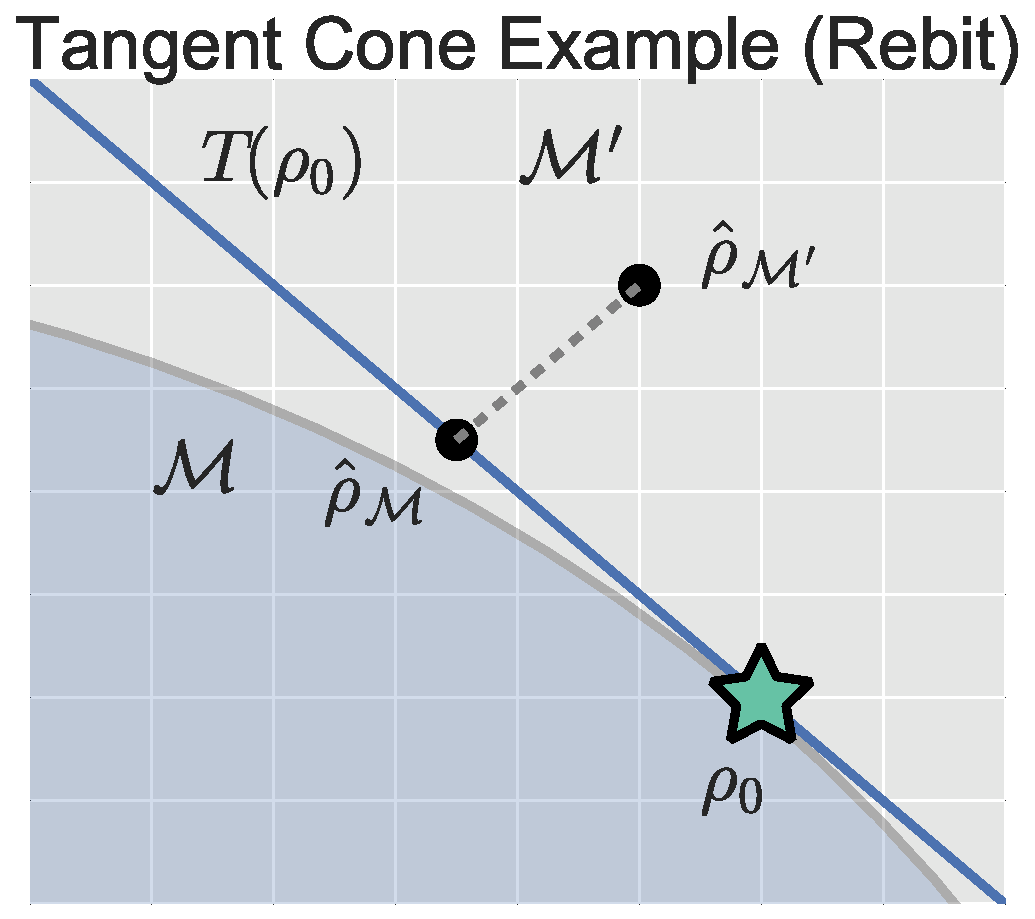
\includegraphics[width=.75\columnwidth]{Images/Figure_temp.pdf}
 \caption{Example of the solid tangent cone for a rebit. As $N_{\mathrm{samples}} \rightarrow \infty$, the local state space around $\rho_{0}$ converges to $T(\rho_{0})$. In Fisher-adjusted coordinates, it's easy to show that $\lambda(\rho_{0}, \M)$ is related to the squared error between $\rhoML{\M}$ and $\rho_{0}$.}
\label{fig:tangentcone}
\end{figure}

Switching back from the Fisher-adjusted coordinates, we have $\lambda(\rho_{0}, \M) = \mathrm{Tr}[(\rho_{0} - \rhoML{\M})\mathcal{I}(\rho_{0} - \rhoML{\M})]$.
~\\~\\
Thus, when LAMPN is satisfied, it's possible to relate the loglikelihood ratio statistic to \emph{squared error} (as measured by the metric induced by $\mathcal{I}$.) This result may be of independent interest in, for example, considering/defining new information criteria, which attempt to balance goodness of fit (as measured by $\lambda$) against error/loss (generally, as measured by the squared error).

With these technical results in hand, we may proceed to compute $\langle \lambda(\M_{d}, \M_{d+1})\rangle$. Doing so is the subject of the next section.

\section{Deriving a Replacement for the Wilks theorem in Tomography}
\label{sec:computingllrs}

With the framework of LAMPN available to us, we are ready to derive a replacement for the Wilks theorem. We first need to show that the models $\M_{d}$ satisfy LAMPN. Thankfully, it is straightforward to do so.

\textbf{Lemma}: The models $\M_{d}$, defined in Equation \eqref{eq:modelsd}, satisfy LAMPN.

\textbf{Proof}: Let $\M'_{d} = \{\sigma ~|~\mathrm{dim}(\sigma) = d, \sigma = \sigma^{\dagger}\}$. (That is, $\M'_{d}$ is the set of all $d \times d$ Hermitian matrices, but we do not require them to be non-negative, nor trace-1.) It is clear $\M_{d} \subset \M'_{d}$. Next, the likelihood $\cL(\sigma)$ is twice continuously differentiable in $\M'_{d}$ at any $\sigma$, meaning $\M'_{d}$ satisfies LAN. Thus, $\M_{d}$ satisfies LAMPN. \qed

As mentioned in the previous section, it's useful to reduce the problem of computing $\lambda(\M_{d}, \M_{d+1})$ to that of computing $\lambda(\rho_{0}, \M_{k})$ for $k = d, d+1$ using the identity
\[\lambda(\M_{d}, M_{d+1}) = \lambda(\rho_{0}, \M_{d+1}) - \lambda(\rho_{0}, \M_{d}).\]
Because each model satisfies LAMPN, it is possible to write $\lambda(\rho_{0}, \M_{k})$ in a very simple form, via Equation \eqref{eq:llrs_lan}:
\[\lambda(\rho_{0}, \M_{k}) = \mathrm{Tr}[(\rho_{0} - \rhoML{\M_{k}})\mathcal{I}_{k}(\rho_{0} - \rhoML{\M_{k}})].\]
The Fisher information $\mathcal{I}_{k}$ is generally anisotropic, and depends on $\rho_{0}$ and the POVM being measured (see Figure \ref{fig:anisofi}). And while the $\rho\geq0$ constraint  that invalidated LAN in the first place is at least somewhat tractable in standard (Hilbert-Schmidt) coordinates, it becomes completely intractable in Fisher-adjusted coordinates.  So, to obtain a semi-analytic null theory for $\lambda$, we will simplify to the case where   $\mathcal{I}_{k} = \Id_{k}/\epsilon $ for some $\epsilon$ that scales as $1/\sqrt{N_{\mathrm{samples}}}$. (That is, $\mathcal{I}_{k}$ is proportional to the Hilbert-Schmidt metric for model $\M_{k}$.) This simplification permits the derivation of analytic results which capture realistic tomographic scenarios surprisingly well \cite{Smolin2012}.
\begin{figure}
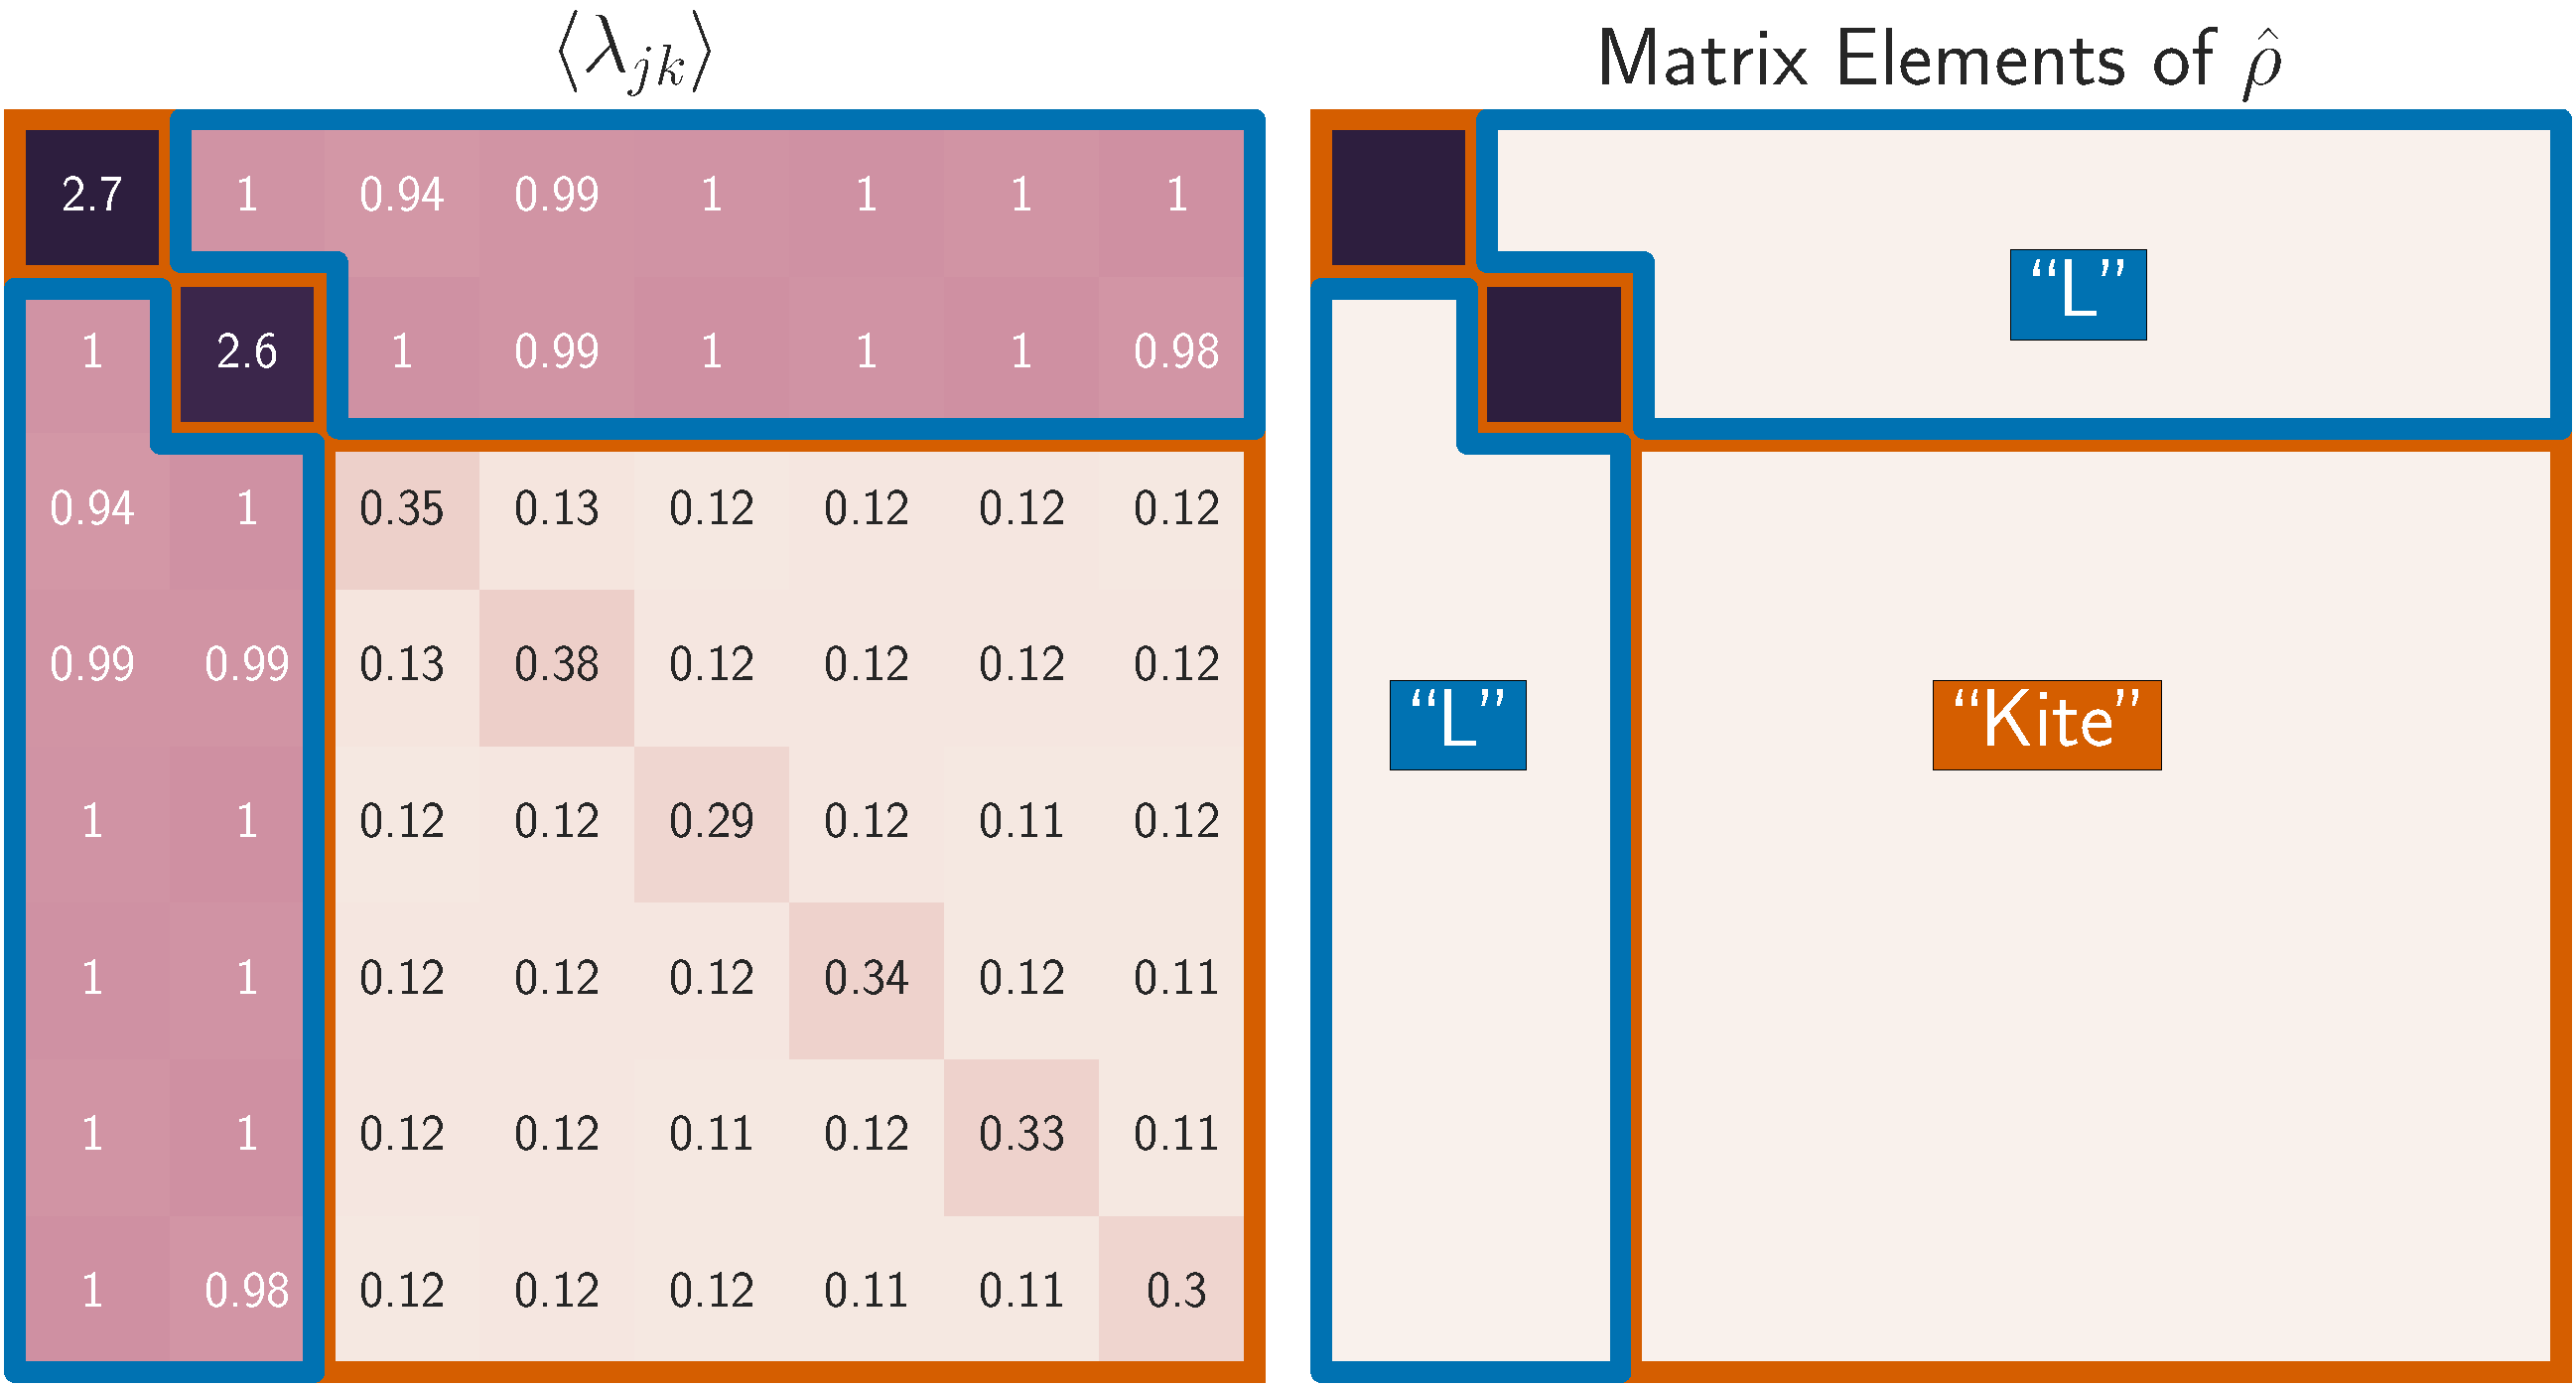
\includegraphics[width=.85\columnwidth]{Images/Figure_2.pdf}
 \caption{Anisotropy of the Fisher information for a rebit measured using the POVM $\frac{1}{2}\{|0\rangle\langle 0|, |1\rangle\langle 1|, |+\rangle\langle +|, |-\rangle\langle -|\}$. Depending on $\rho_{0}$ (star), the distribution of the unconstrained estimates $\hat{\rho}_{\mathrm{ML}}$ (ellipses) may be anisotropic. Imposing the positivity constraint $\rho \geq 0$ is difficult in Fisher-adjusted coordinates; in this paper, we simplify these complexities to the case where $\mathcal{I} \propto \Id$, \emph{and is independent of $\rho_{0}$}.}
\label{fig:anisofi}
\end{figure}

With this simplification, $\lambda(\M_{d},\M_{d+1})$ is given by
\begin{equation}
\lambda = \frac{1}{\epsilon^{2}}\left(\mathrm{Tr}[(\rho_{0} - \rhoML{d+1})^{2}] -  \mathrm{Tr}[(\rho_{0} - \rhoML{d})^{2}]\right).
\end{equation}
That is, $\lambda$ is a \emph{difference} in Hilbert-Schmidt distances. This expression makes it clear why a null theory for $\lambda$ is necessary: even if $\rho_{0} \in \M_{d},\M_{d+1}$, the error of $\rhoML{d+1}$ will be greater than that of $\rhoML{d}$ (because there are more parameters which can fit noise in the data); to know if $\M_{d+1}$ is actually fitting additional \emph{structure} in the data, we need to know how much noise we would erroneously accept as structure.

In computing $\mathrm{Pr}(\lambda)$ we face the obstacle that the distributions of $\rhoML{d}, \rhoML{d+1}$ are complicated, highly non-Gaussian, and singular (because estimates ``pile up'' on the various faces of the boundary; recall Figure \ref{fig:boundaries}).  For this reason, we will not attempt to compute $\mathrm{Pr}(\lambda)$ directly.  Instead, we focus on deriving a good approximation for $\langle \lambda \rangle$.

Because $\expect{\lambda}$ itself depends on two terms, each of which has a similar form, we can further simplify our task to that of computing $\epsilon^{2}\langle \lambda(\rho_{0}, \M_{d}) \rangle = \langle \mathrm{Tr}[(\rhoML{d}  - \rho_{0})^{2}] \rangle$ for arbitrary $d$.
Doing so involves two main steps:
\begin{itemize}
\item[(1)] Identifying degrees of freedom in $\rhoML{\M'_{d}}$ that are unaffected by projection onto the tangent cone $T(\rho_{0})$, and those that are.
\item[(2)] For both types of degrees of freedom, evaluate the contributions of each degree of freedom to the value of $\langle \lambda \rangle$.
\end{itemize}

The remainder of this section is devoted to doing both steps. In Section \ref{subsec:dof}, we identify two types of degrees of freedom in $\rhoML{\M'}$, which we call the ``L" and the ``kite", respectively. Section \ref{subsec:L} computes the contribution of degrees of freedom in the ``L", and Section \ref{subsec:kite} computes the contribution from the ``kite". The total expected value is given in Equation \eqref{eq:ourLLRS} in Section \ref{subsec:LLRS}.

\subsection{Separating out Degrees of Freedom in $\rhoML{\M'_{d}}$}
\label{subsec:dof}
We begin by observing that $\lambda(\rho_{0}, \M_{d})$ can be written as a sum over matrix elements,
\begin{align}
\label{eq:llrserrors}
\nonumber \lambda &=\epsilon^{-2}\mathrm{Tr}[(\rhoML{d} - \rho_{0})^{2}] = \epsilon^{-2}\sum_{jk}|(\rhoML{d}- \rho_{0} )_{jk}|^{2}\\
&= \sum_{jk}\lambda_{jk}~~~~\text{where}~~~~\lambda_{jk} = \epsilon^{-2}|(\rhoML{d} - \rho_{0} )_{jk} |^{2},
\end{align}
and therefore $\langle \lambda \rangle = \sum_{jk}\langle\lambda_{jk}\rangle$.  Each term $\langle \lambda_{jk}\rangle$ quantifies the mean-squared error of a single matrix element of $\rhoML{d}$, and while the Wilks theorem predicts $\expect{\lambda_{jk}}=1$ for all $j,k$, due to positivity constraints, this no longer holds. In particular, the matrix elements of $\rhoML{d}$ now fall into two parts:

\begin{enumerate}[noitemsep]
\item Those for which the corresponding matrix elements of $\rhoML{\M'_{d}}$ \emph{are constrained}.
\item Those for which the corresponding matrix elements of $\rhoML{\M'_{d}}$ \emph{are not constrained}, because they correspond to directions on the surface of the tangent cone $T(\rho_{0})$.
\end{enumerate}
This division is a natural one, given LAMPN - even after projection onto $T(\rho_{0})$, some matrix elements of $\rhoML{\M_{d}}$ will not be constrained, while others will. (Recall Figure \ref{fig:tangentcone} - as a component of $\rhoML{\M'}$ along $T(\rho_{0})$ changes, the component of $\rhoML{\M}$ changes by the same amount. These elements are unconstrained.) The former, which lie in what we call the ``L", comprise all off-diagonal elements on the support of $\rho_0$ \emph{and} between the support and the kernel, while the latter, which lie in what we call the ``kite", are all diagonal elements \emph{and} all elements on the kernel (null space) of $\rho_0$.

Performing this division is also supported by numerical simulations (see Figure \ref{fig:L}). Matrix elements in the ``L" appear to contribute $\langle \lambda_{jk}\rangle = 1$, consistent with the Wilks theorem, while those in the ``kite" contribute more (if they are within the support of $\rho_{0}$) or less (if they are in the kernel).  Having performed the division of the matrix elements of $\rhoML{\M'_{d}}$, we observe that $\langle\lambda\rangle = \expect{\lambda_{\mathrm{L}}} + \expect{\lambda_{\mathrm{kite}}}$. Because each $\langle \lambda_{jk}\rangle$ is not necessarily equal to one (as in the Wilks theorem), and because many of them are less than 1, it's clear that their total $\langle \lambda \rangle$ is dramatically lower than that predicted by the Wilks theorem. (Recall Figure \ref{fig:boundaries2}.)

\begin{figure}[h]
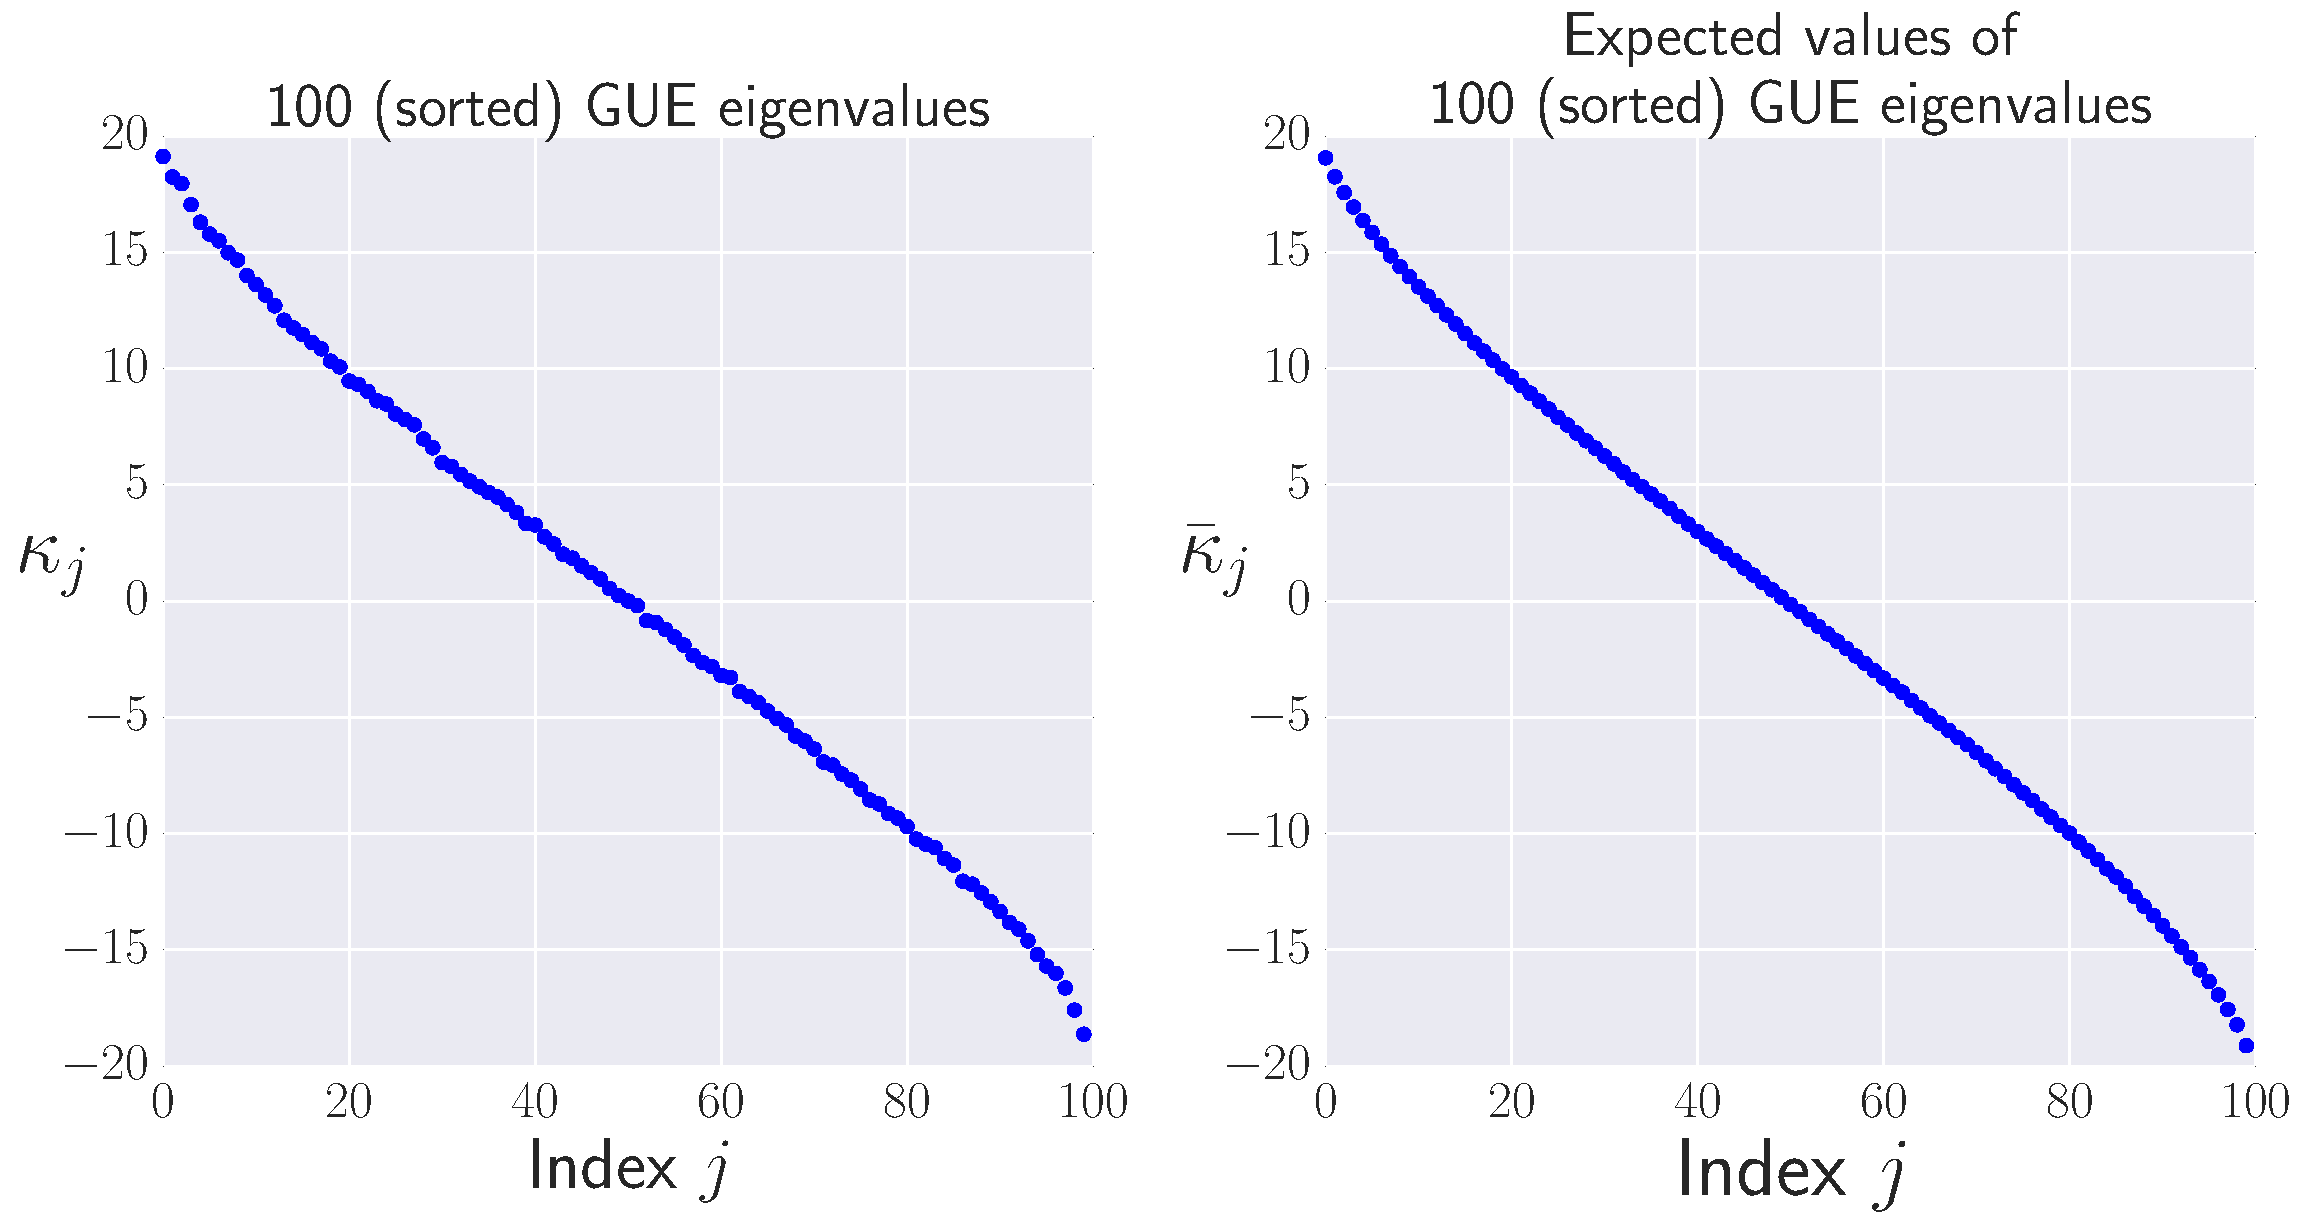
\includegraphics[width=\columnwidth]{Images/Figure_3.pdf}
 \caption{When a rank-2 state is reconstructed in $d=8$ dimensions, the total loglikelihood ratio $\lambda(\rho_0,\mathcal{M}_8)$ is the sum of terms $\lambda_{jk}$ from errors in each matrix element $(\rhoML{d})_{jk}$.  \textbf{Left}:  Numerics show a clear division; some matrix elements have $\expect{\lambda_{jk}}\sim1$ as predicted by the Wilks theorem, while others are either more or less. \textbf{Right}:  The numerical results support our theoretical reasoning for dividing the matrix elements of $\rhoML{\M'_{d}}$ into two parts: the ``kite'' and the ``L''.}
\label{fig:L}
\end{figure}

In the following subsections, we develop a theory to explain the behavior of $\langle \lambda_{\mathrm{L}}\rangle$ and \expect{\lambda_{\mathrm{kite}}}.
In doing so, it is helpful to think about the error of the unconstrained estimate $\delta \equiv \rhoML{\M'_{d}}- \rho_{0}$, a normally-distributed \emph{traceless} matrix.  To simplify the analysis, we explicitly drop the $\Tr(\delta)=0$ constraint and let $\delta$ be $\mathcal{N}(0,\epsilon^2\Id)$ distributed over the $d^2$-dimensional space of Hermitian matrices (a good approximation when $d\gg2$) \footnote{That is, we let $\mathrm{Tr}(\delta)$ fluctuate as well.}, which makes $\delta$ proportional to an element of the Gaussian Unitary Ensemble (GUE) \cite{Fyodorov2005}.

\subsection{Computing $\langle \lambda_\mathrm{L}\rangle$}
\label{subsec:L}
Elements of $\delta$ in the ``L'' are unconstrained by the boundary (the surface of the tangent cone $T(\rho_{0})$), and behave exactly as expected from classical theory.  Because $\M'$ satisfies LAN, it follows that each component is an i.i.d. Gaussian random variable. Thus, for each element of $\delta$ in the ``L", we have $(\rhoML{\M_{d}})_{jk} = (\rhoML{\M'_{d}})_{jk}$, and $\langle \lambda_{jk} \rangle = \langle \delta_{jk}^{2}\rangle /\epsilon^{2} = 1$. The surface of the tangent cone is $2rd - r(r+1)$-dimensional, so $\expect{\lambda_{\mathrm{L}}} = 2rd - r(r+1)$.
\todo[inline]{Should we explicitly call out the dimension as being related to the dimension of the manifold of rank-$r$ states in $d$-dimensions?}
Another way of viewing this result is to observe that the $\delta_{jk}$ in the ``L'' can be seen as errors which arise due to small unitary perturbations of $\rho_{0}$. Writing $\rhoML{\M'_{d}} = U^{\dagger}\rho_{0}U$, where $U=e^{i\epsilon H}$, we have
\[\rhoML{\M'_{d}} \approx \rho_{0} + i\epsilon [\rho_{0},H]+\mathcal{O}(\epsilon^{2}).\]
Then, $\delta \approx i\epsilon [\rho_{0},H]$.
If $j = k$, then $\delta_{jj} = 0$. Thus, small unitaries cannot create errors in the diagonal matrix elements, at $\mathcal{O}(\epsilon)$. If $j \neq k$, then $\delta_{jk} \neq 0$, in general. (Small unitaries \emph{can} introduce errors on off-diagonal elements.)

However, if either $j$ or $k$ (or both) lie within the \emph{kernel} of $\rho_{0}$ (i.e., $\langle k | \rho_{0}| k \rangle$ or $\langle j|\rho_{0}|j\rangle$ is 0), then the corresponding $\delta_{jk}$ are zero. The only off-diagonal elements where small unitaries can introduce errors are those which are coherent between the kernel of $\rho_{0}$ and its support. These off-diagonal elements are precisely the ``L", and are  the set $\{\delta_{jk}~|~\langle j | \rho_{0}|j\rangle \neq 0, j\neq k, ~ 0 \leq j,k \leq d - 1\}$. This set contains $2rd - r(r+1)$ elements, each of which has $\langle \lambda_{jk}\rangle = 1$, so we again arrive at $\expect{\lambda_{\mathrm{L}}} = 2rd - r(r+1)$.

\subsection{Computing $\langle \lambda_\mathrm{kite}\rangle$}
\label{subsec:kite}
Computing $\langle \lambda_{\mathrm{L}}\rangle$ was made easy by the fact that the matrix elements of $\delta$ in the ``L" are unaffected by the projection of $\rhoML{\M'_{d}}$ onto $T(\rho_{0})$. Computing $\expect{\lambda_{\mathrm{kite}}}$ is a bit harder, because the boundary \emph{does} constrain its elements. We need a procedure to compute $\rhoML{d}$ given $\rhoML{\M'_{d}}$ -- i.e., to solve the optimization problem in Eq. \eqref{eq:lampnmle}.  Fortunately, an algorithm for doing so was presented in \cite{Smolin2012}:
\begin{enumerate}[noitemsep]
\item Subtract $q\Id$ from $\rhoML{\M'_{d}}$, for a particular real scalar $q$.
\item ``Truncate'' $\rhoML{\M'_{d}}-q\Id$, by replacing each of its negative eigenvalues with zero.
\end{enumerate}
Here, $q$ is defined implicitly such that $\Tr\left[ \mathrm{Trunc}(\rhoML{\M'_{d}}-q\Id)\right] = 1$.

Although this was intended as a very fast numerical algorithm, we will manipulate it (by a series of approximations) to derive a closed-form, deterministic approximation for $q$. (While it is true $q$ is a random variable -- after all, it depends on $\rhoML{\M'_{d}}$ -- it turns out that the \emph{typical} behavior of $q$ is relevant for computing $\langle \lambda_{\mathrm{kite}}\rangle$.)

The truncation algorithm given in \cite{Smolin2012} for finding $\rhoML{d}$ is most naturally performed in the eigenbasis of $\rhoML{\M'_{d}}$.  Exact diagonalization of $\rhoML{\M'_{d}}$ is not feasible analytically, but only its \emph{small} eigenvalues are critical in truncation.  We assume that $N_{\mathrm{samples}}$ is sufficiently large so that all the nonzero eigenvalues of $\rho_0$ are much larger than $\epsilon$. This means the eigenbasis of $\rhoML{\M'_{d}}$ is accurately approximated by: (1) 
the eigenvectors of $\rho_0$ on its support; and (2) the eigenvectors of $\delta_{\mathrm{ker}} = \Pi_{\mathrm{ker}}\delta\Pi_{\mathrm{ker}}$, where $\Pi_{\mathrm{ker}}
$ is the projector onto the kernel of $\rho_0$.

Changing to this basis diagonalizes the ``kite'' portion of $\delta$, and leaves all elements of the ``L'' unchanged (at $\mathcal{O}(\epsilon)$).  The diagonal elements of $\rhoML{\M'_{d}}$ now fall into two categories:
\begin{enumerate}[noitemsep]
\item $r$ elements corresponding to the eigenvalues of $\rho_0$, which are given by $p_{j} = \rho_{jj} + \delta_{jj}$ where  $\rho_{jj}$ is the $j^{\mathrm{th}}$ eigenvalue of $\rho_{0}$, and $\delta_{jj} \sim \mathcal{N}(0,\epsilon^2)$.
\item $N \equiv d-r$ elements that are eigenvalues of $\delta_{\mathrm{ker}}$, which we denote by $\bvec{\kappa} = \{\kappa_j:~j = 1\ldots 
N\}$,
\end{enumerate}
and $\lambda_{\mathrm{kite}}$ is
\begin{equation}
\label{eq:llrs_kite}
\epsilon^{2}\lambda_{\mathrm{kite}} = \sum_{j=1}^{r}[\rho_{jj}- (p_j-q)^{+}]^2 + \sum_{j=1}^{N}\left[(\kappa_j-q)^+\right]^2,
\end{equation}
where $(x)^{+} = \max(x, 0)$. $q$ is implicitly defined such that $\Tr\left[\mathrm{Trunc}(\rhoML{\M'_{d}} - q \Id)\right] = 1$. In terms of the eigenvalues of $\rhoML{\M'_{d}}$, this means $q$ is the solution to
\begin{equation}
\label{eq:q_eqn}
 \sum_{j=1}^{r}(p_j - q)^{+} + \sum_{j=1}^{N}{(\kappa_j-q)^+} = 1.
\end{equation}

To solve Equation \eqref{eq:q_eqn}, and derive an approximation for \eqref{eq:llrs_kite}, we need to understand the behavior of $\bvec{\kappa}$. It is to this problem we now turn.

\subsubsection{Approximating the Eigenvalues of a GUE($N$) Matrix}
We first observe that while the $\kappa_j$ are random variables, they are \emph{not} normally distributed.  Instead, because $\delta_{\mathrm{ker}}$ is proportional to a $\mathrm{GUE}(N)$ matrix, for $N\gg1$, the distribution of any eigenvalue $\kappa_{j}$
converges to a Wigner semicircle distribution \cite{Wigner1958}, given by $\mathrm{Pr}(\kappa) = \frac{2}{\pi R^{2}}\sqrt{R^{2}-\kappa^{2}}$ for $|\kappa| \leq R$, with $R = 2\epsilon\sqrt{N}$.  The eigenvalues are not independent; they tend to avoid collisions (``level avoidance'' \cite{Tao2013}), 
and typically form a surprisingly regular array over the support of the Wigner semicircle.  Since our goal is to compute $\expect{\lambda_{\mathrm{kite}}}$, we can capitalize on this behavior by replacing each random sample of $\bvec{\kappa}$ with a 
\emph{typical sample} $\bar{\bvec{\kappa}}$ given by its order statistics.  These are the average values of the \emph{sorted} 
$\bvec{\kappa}$, so $\overline{\kappa}_j$ is the average value of the $j^{\mathrm{th}}$ largest value of $\bvec{\kappa}$.  Large random samples 
are usually well approximated (for many purposes) by their order statistics even when the elements of the sample are 
independent, and level avoidance makes the approximation even better. 

\begin{figure}[h!]
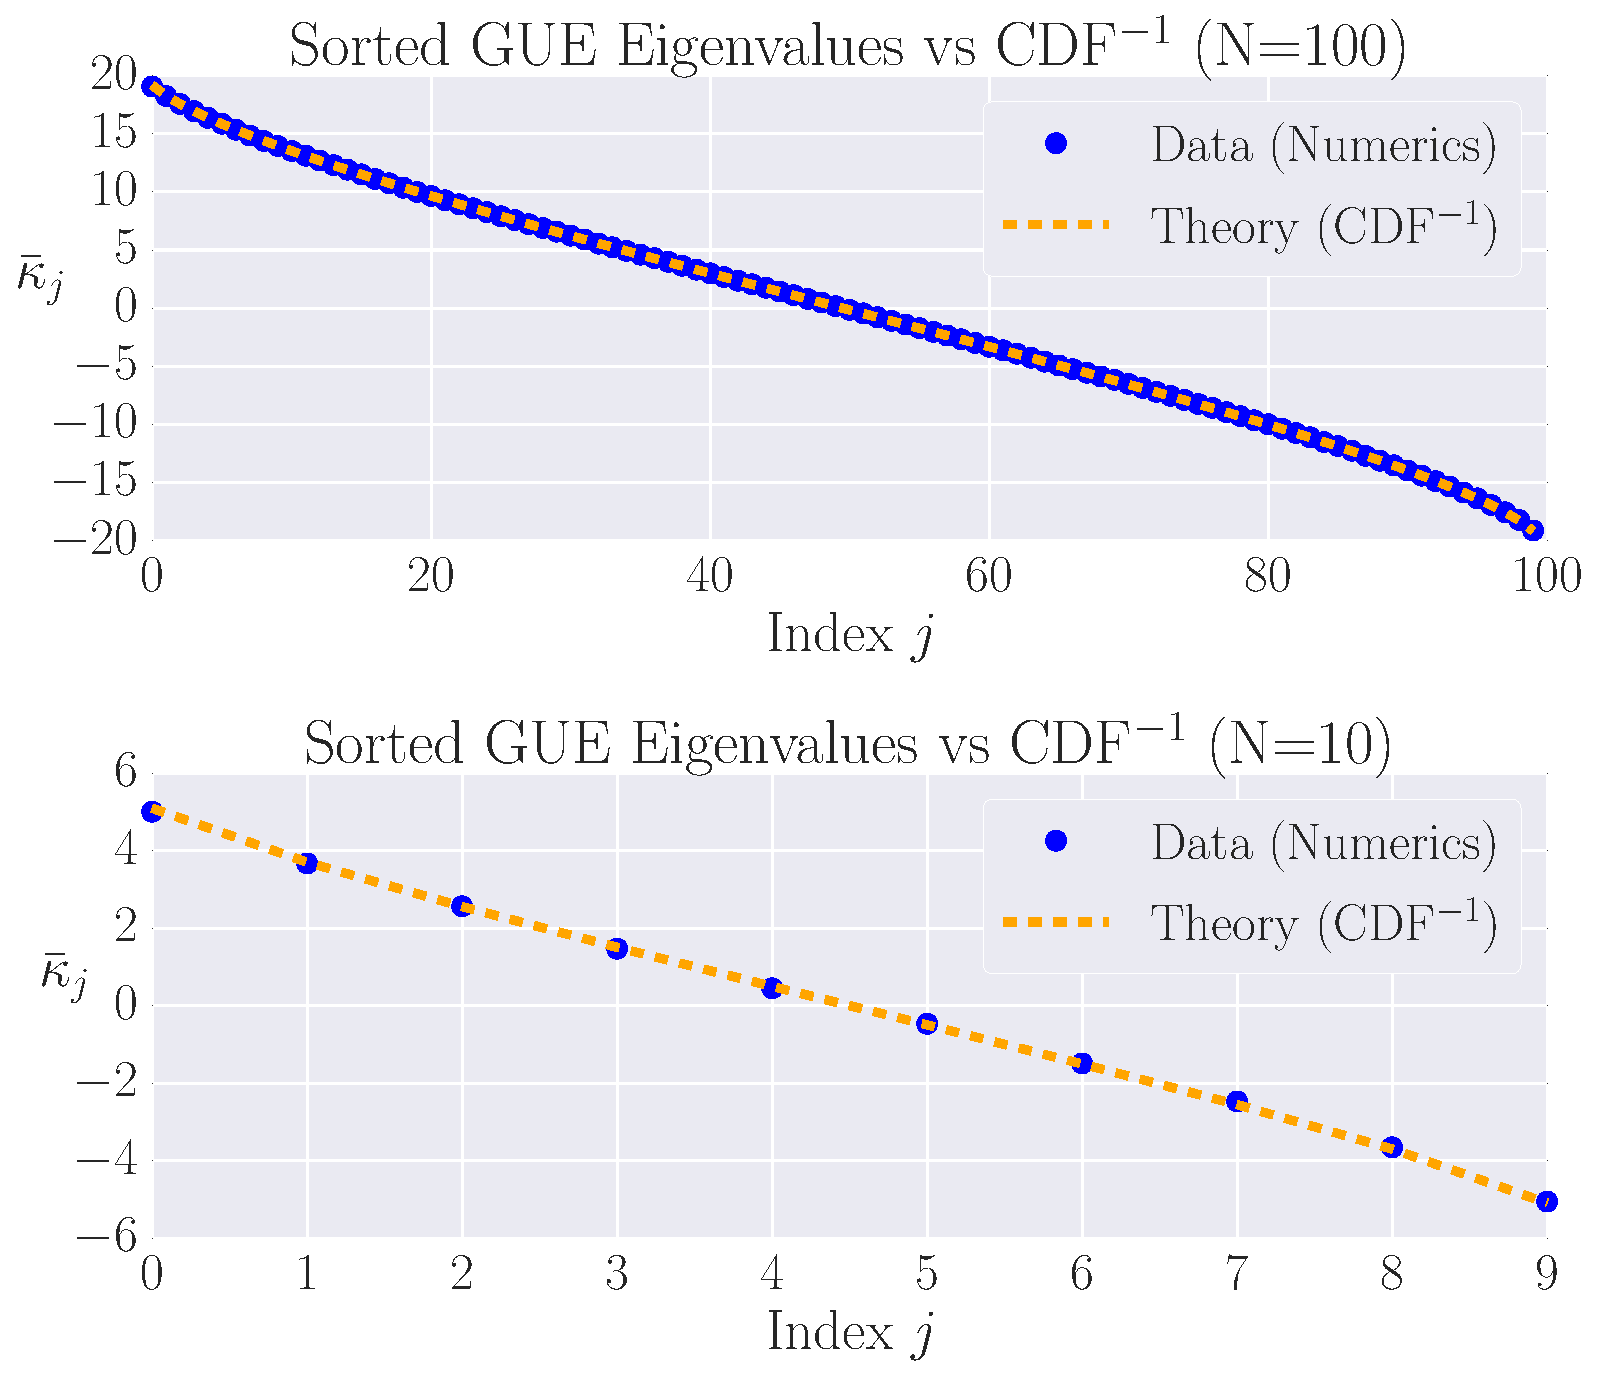
\includegraphics[width=\columnwidth]{Images/Figure_4.pdf}
\caption{Typical samples of GUE($N$) eigenvalues are accurately approximated by order statistics of the distribution (average values of a sorted sample).  \textbf{Left}:  The sorted eigenvalues (i.e., order statistics $\kappa_{j}$) of one randomly chosen GUE(100) matrix.  \textbf{Right}:  Approximate expected values of the order statistics, $\bar{\kappa}_{j}$, of the GUE(100) distribution, computed as the average of the sorted eigenvalues of 100 randomly chosen GUE(100) matrices.}
\label{fig:orderstatistics1}
\end{figure}

Suppose that $\bvec{\kappa}$ are the eigenvalues of a GUE($N$) matrix, sorted from highest to lowest.  Figure \ref{fig:orderstatistics1} illustrates such a sample for $N=100$.  It also shows the \emph{average} values of 100 such samples (all sorted).  These are the \emph{order statistics} $\overline{\bvec{\kappa}}$ of the distribution (more precisely, what is shown is a good \emph{estimate} of the order statistics; the actual order statistics would be given by the average over infinitely many samples).  The point of the figure is to show that, while the order statistics \emph{are} slightly more smoothly and predictably distributed than a single (sorted) sample, the two are remarkably similar.  A single sample $\bvec{\kappa}$ will fluctuate around the order statistics, but these fluctuations are relatively small, partly because the sample is large, and partly because the GUE eigenvalues experience level repulsion.  Thus, the ``typical'' behavior of a sample -- by which we mean the mean value of a statistic of the sample -- is well captured by the order statistics (which have no fluctuations at all).

We now turn to the problem of modeling $\bvec{\kappa}$ quantitatively.  We note up front that we are only going to be interested in certain properties of $\bvec{\kappa}$:  specifically, partial sums of all $\kappa_j$ greater or less than the threshold $q$, or partial sums of functions of the $\kappa_j$ (e.g. $(\kappa_j-q)^2$).  We require only that an ansatz be accurate for such quantities.  We do not use this fact explicitly, but it motivates our approach -- and we do not claim that our ansatz is accurate for \emph{all} conceivable functions.

In general, if a sample $\bvec{\kappa}$ of size $N$ is drawn so that each $\kappa$ has the same probability density 
function $\mathrm{Pr}(\kappa)$, then a good approximation for the $j^{\mathrm{th}}$ order statistic is given by the inverse 
\emph{cumulative} distribution function (CDF):
\begin{equation}
\overline{\kappa}_j \approx \mathrm{CDF}^{-1}\left(\frac{j-1/2}{N}\right).
\end{equation}
This is closely related to the observation that the histogram of a sample tends to look similar to the underlying probability density function.  More precisely, it is equivalent to the observation that the empirical distribution function (the CDF of the histogram) tends to be (even more) similar to the underlying CDF.  (For i.i.d. samples, this is the content of the Glivenko-Cantelli theorem \cite{VanderVaart2000}).  Figure \ref{fig:orderstatistics2} compares the order statistics of GUE(100) and GUE(10) eigenvalues (computed as numerical averages over 100 random samples) to the inverse CDF for the Wigner semicircle distribution.  Even though the Wigner semicircle model of GUE eigenvalues is only exact as $N\to\infty$, it provides a nearly-perfect model for $\overline{\bvec{\kappa}}$ even at $N=10$ (and remains surprisingly good all the way down to $N=2$).

\begin{figure}[h!]
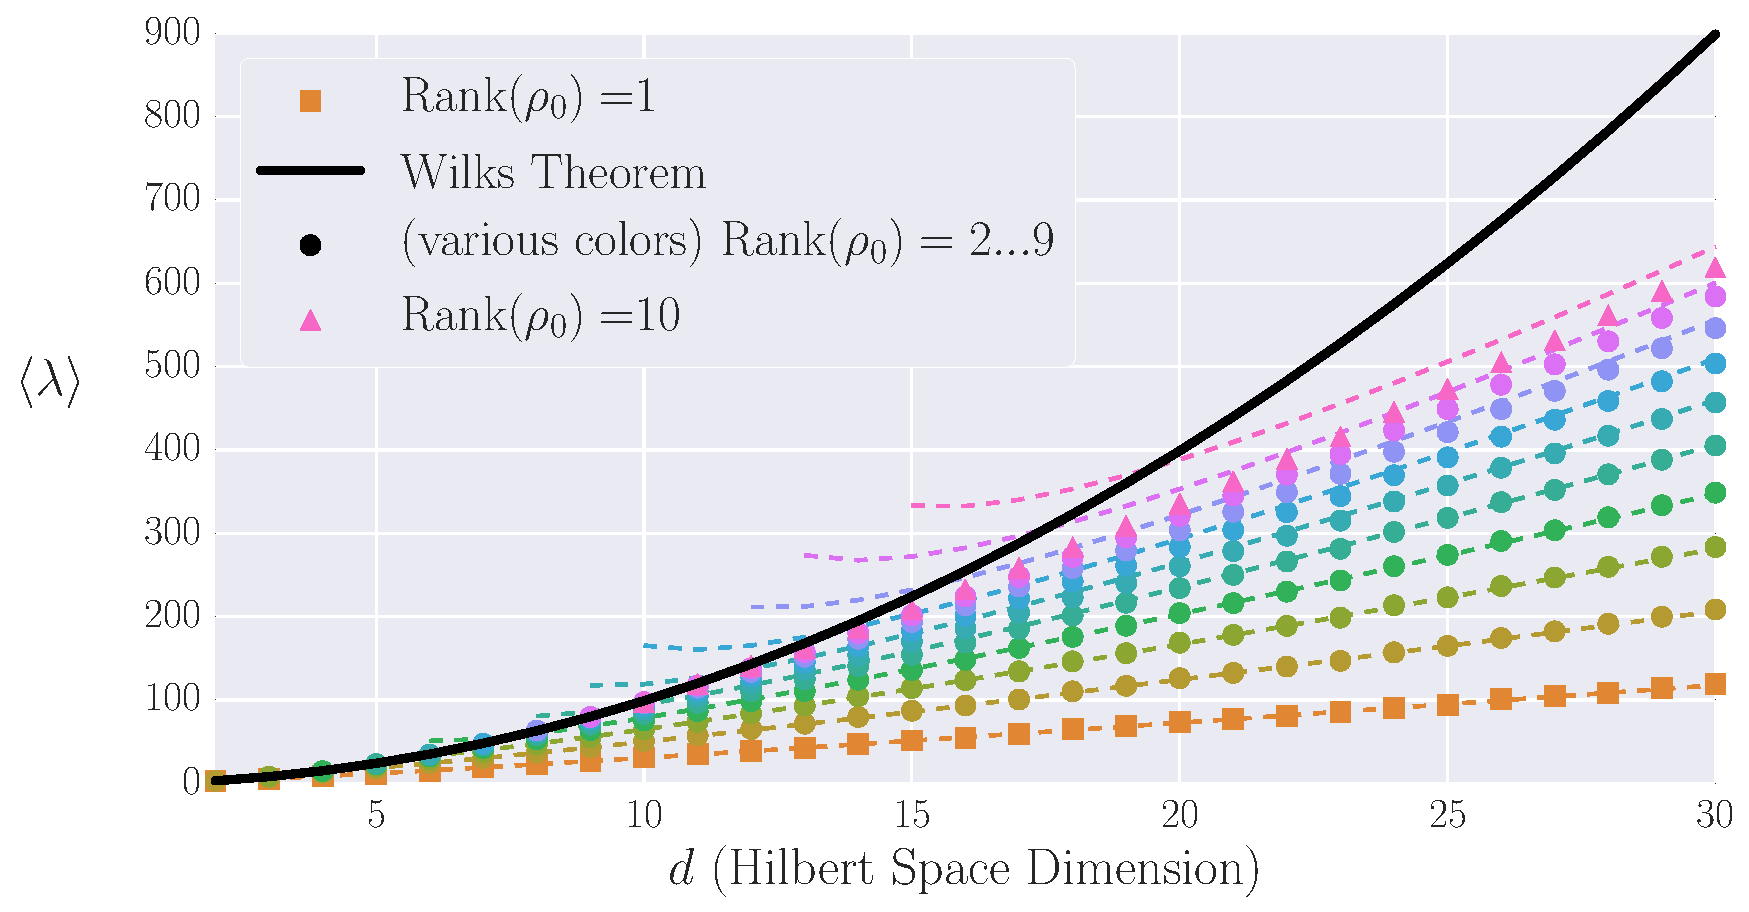
\includegraphics[width=\columnwidth]{Images/Figure_5.pdf}
\caption{Order statistics of the GUE($N$) eigenvalue distribution are very well approximated by the inverse CDF of the Wigner semicircle distribution.  In both figures, we compare the order statistics of a GUE($N$) distribution to the inverse CDF of the Wigner semicircle distribution. \textbf{Top}:  $N=100$.  \textbf{Bottom}:  $N=10$.
Agreement in both cases is essentially perfect.}
\label{fig:orderstatistics2}
\end{figure}

We make one further approximation, by assuming that $N\gg1$, so the distribution of the $\overline{\kappa}_j$ is effectively continuous and identical to $\mathrm{Pr}(\kappa)$. For the quantities that we compute, this is equivalent to replacing the empirical distribution function (which is a step function) by the CDF of the Wigner semicircle distribution.  So, whereas for any given sample the partial sum of all $\kappa_j > q$ jumps discontinuously when $q=\kappa_j$ for any $j$, in this approximation it changes smoothly.  This accurately models the \emph{average} behavior of partial sums.

\subsubsection{Deriving an Approximation for $q$}
The approximations of the previous section allow us to use the following ansatz for the eigenvalues of $\rhoML{\M'_{d}}$; namely, $\{p_j\} \cup \{\overline{\kappa}_j\}$, where the $p_j$ are $\mathcal{N}(\rho_{jj},\epsilon^2)$ random variables, and the $\overline{\kappa}_j$ are the (fixed, smoothed) order statistics of a Wigner semicircle distribution.  In turn, the defining equation for $q$ (Equation \eqref{eq:q_eqn}) is well approximated as
\begin{equation}
\sum_{j=1}^{r}(p_j - q)^{+} + \sum_{j=1}^{N}{(\overline{\kappa}_j-q)^+} \approx 1.
\end{equation}
To solve this equation, we observe that the $\overline{\kappa}_j$ are symmetrically distributed around $
\kappa=0$, so half of them are negative.  Therefore, with high probability, $\Tr
\left[\mathrm{Trunc}(\rhoML{\M'_{d}})\right]>1$, and so we will need to subtract $q\Id$ from $\rhoML{\M'_{d}}$ before truncating.

Because we have assumed $N_{\mathrm{samples}}$ is sufficiently large ($N_{\mathrm{samples}} >> \min_{j}1/\rho_{jj}^{2}$), it follows that the eigenvalues of $\rho_{0}$ are large compared to the perturbations $\delta_{jj}$ and $q$. This implies $(p_{j} - q)^{+} = p_{j} - q$. Under this assumption, $q$ is the solution to
\begin{align}
\nonumber 1 &\approx \sum_{j=1}^{r}(p_j - q)^{+} + \sum_{j=1}^{N}{(\overline{\kappa}_j-q)^+}\\
\nonumber &\approx 1 - rq + \Delta + N\int_{\kappa=q}^{2\epsilon\sqrt{N}}{(\kappa-q)\mathrm{Pr}(\kappa)\mathrm{d}\kappa}\\
\label{eq:q_eqn2}\implies 0 &= - rq + \Delta + \frac{\epsilon}{12\pi}\left[
\begin{array}{l} (q^2+8N)\sqrt{-q^2+4N} \\
-12qN\left(\frac{\pi}{2}-\sin^{-1}\left(\frac{q}{2\sqrt{N}}\right)\right)
\end{array}\right],\nonumber\\
~
\end{align}
where $\Delta = \sum_{j=1}^{r}\delta_{jj}$ is a $\mathcal{N}(0,r\epsilon^2)$ random variable.  We choose to replace a discrete 
sum (line 1) with an integral (line 2). This approximation is valid when $N\gg1$, as we can accurately approximate a discrete collection of closely spaced real numbers by a smooth density or distribution over the real numbers that has approximately the same CDF.  It is also remarkably accurate in practice.
  
In yet another approximation, we replace $\Delta$ with its average value, which is zero.  We could obtain an even more accurate expression 
 by treating the fluctuations in $\Delta$ more carefully, but this crude approximation turns out to be quite accurate already.

To solve Equation \eqref{eq:q_eqn2}, it is necessary to further simplify the complicated expression resulting from the integral (line 3).  To do so, we 
assume  $\rho_0$ is relatively low-rank, so $r \ll N$.  In this case, the sum of the positive $\overline{\kappa}_j$ is large compared 
with $r$, almost all of them need to be subtracted away, and therefore $q$ is close to $2\epsilon\sqrt{N}$.  \footnote{This justifies the assumption that $\rho_{jj} + \delta_{jj} - q > 0$.} We therefore replace 
the complicated expression with its leading order Taylor expansion around $q=2\epsilon\sqrt{N}$, substitute into Equation \eqref{eq:q_eqn2}, and 
obtain the equation
\begin{equation}
\frac{rq}{\epsilon}  = \frac{4}{15\pi}N^{1/4}\left(2\sqrt{N}-\frac{q}{\epsilon}\right)^{5/2}.
\end{equation}
This equation is a quintic polynomial, so it has no closed-form solution.  However, its roots have a well-defined asymptotic ($N\to
\infty$) expansion that becomes accurate quite rapidly (e.g., for $N>4$):
\begin{equation}
\label{eq:truncation}
z \equiv q/\epsilon \approx 2\sqrt{N}-\frac{(240r\pi)^{2/5}}{4}N^{1/10}+\frac{(240r\pi)^{4/5}}{80}N^{-3/10}.
\end{equation}

\subsubsection{Expression for $\langle \lambda_{\mathrm{kite}}\rangle$}
Now that we know how much to subtract off in the truncation process, we can approximate $\expect{\lambda_{\mathrm{kite}}}$, originally given in Equation \eqref{eq:llrs_kite}:
\begin{align}
\nonumber \expect{\lambda_{\mathrm{kite}}} &\approx  \frac{1}{\epsilon^{2}}\left\langle\sum_{j=1}^{r}[\rho_{jj}- (p_j-q)^{+}]^2 + \sum_{j=1}^{N}\left[(\bar{\kappa}_j-q)^+\right]^2 \right\rangle\\
\nonumber &\approx \frac{1}{\epsilon^{2}} \left\langle\sum_{j=1}^{r}[-\delta_{jj} +  q ]^2 + \sum_{j=1}^{N}\left[(\bar{\kappa}_j-q)^+\right]^2 \right\rangle\\
\nonumber  &\approx r + rz^2 + \frac{N}{\epsilon^{2}}\int_{\kappa=q}^{2\epsilon\sqrt{N}}{ \mathrm{Pr}(\kappa)(\kappa-q)^2 d\kappa} \\
\nonumber &=r + rz^{2} + \frac{N(N+z^{2})}{\pi}\left(\frac{\pi}{2} - \sin^{-1}\left(\frac{z}{2\sqrt{N}}\right)\right) \\
& - \frac{z(z^{2}+26N)}{24\pi}\sqrt{4N-z^{2}}.
\end{align}

\subsection{Complete Expression for $\langle \lambda \rangle$}
\label{subsec:LLRS}
The total expected value, $\expect{\lambda} = \expect{\lambda_{\mathrm{L}}} + \expect{\lambda_{\mathrm{kite}}}$, is thus
\begin{align}
\label{eq:ourLLRS}
\nonumber \langle \lambda(\rho_{0}, \M_{d}) \rangle &\approx 2rd - r^{2}+rz^{2}\\
\nonumber & + \frac{N(N+z^{2})}{\pi}\left(\frac{\pi}{2} - \sin^{-1}\left(\frac{z}{2\sqrt{N}}\right)\right) \\
& - \frac{z(z^{2}+26N)}{24\pi}\sqrt{4N-z^{2}}.
\end{align}
where $z$ is given in Equation \eqref{eq:truncation}, $N=d-r$, and $r = \mathrm{Rank}(\rho_{0})$.

\section{Comparison to Numerical Experiments}

\subsection{Isotropic Fisher Information}
\label{sec:theorycomp1}

Equation \eqref{eq:ourLLRS} is our main result.  To test its validity, we compare it to numerical simulations for the case of an isotropic Fisher information
with $d=2,\ldots,30$ and $r=1,\ldots,10$ in Figure \ref{fig:modelcomp-iso}.  The prediction of the Wilks theorem is wildly incorrect for $r\ll d$. In contrast, Equation \eqref{eq:ourLLRS} is almost perfectly accurate when $r \ll d$, but it does begin to break down (albeit fairly gracefully) as $r$ becomes comparable to $d$.  We conclude that our analysis (and Equation \eqref{eq:ourLLRS}) correctly models tomography \emph{if} the Fisher information is isotropic ($\Fi \propto \Id$).

\begin{figure}
 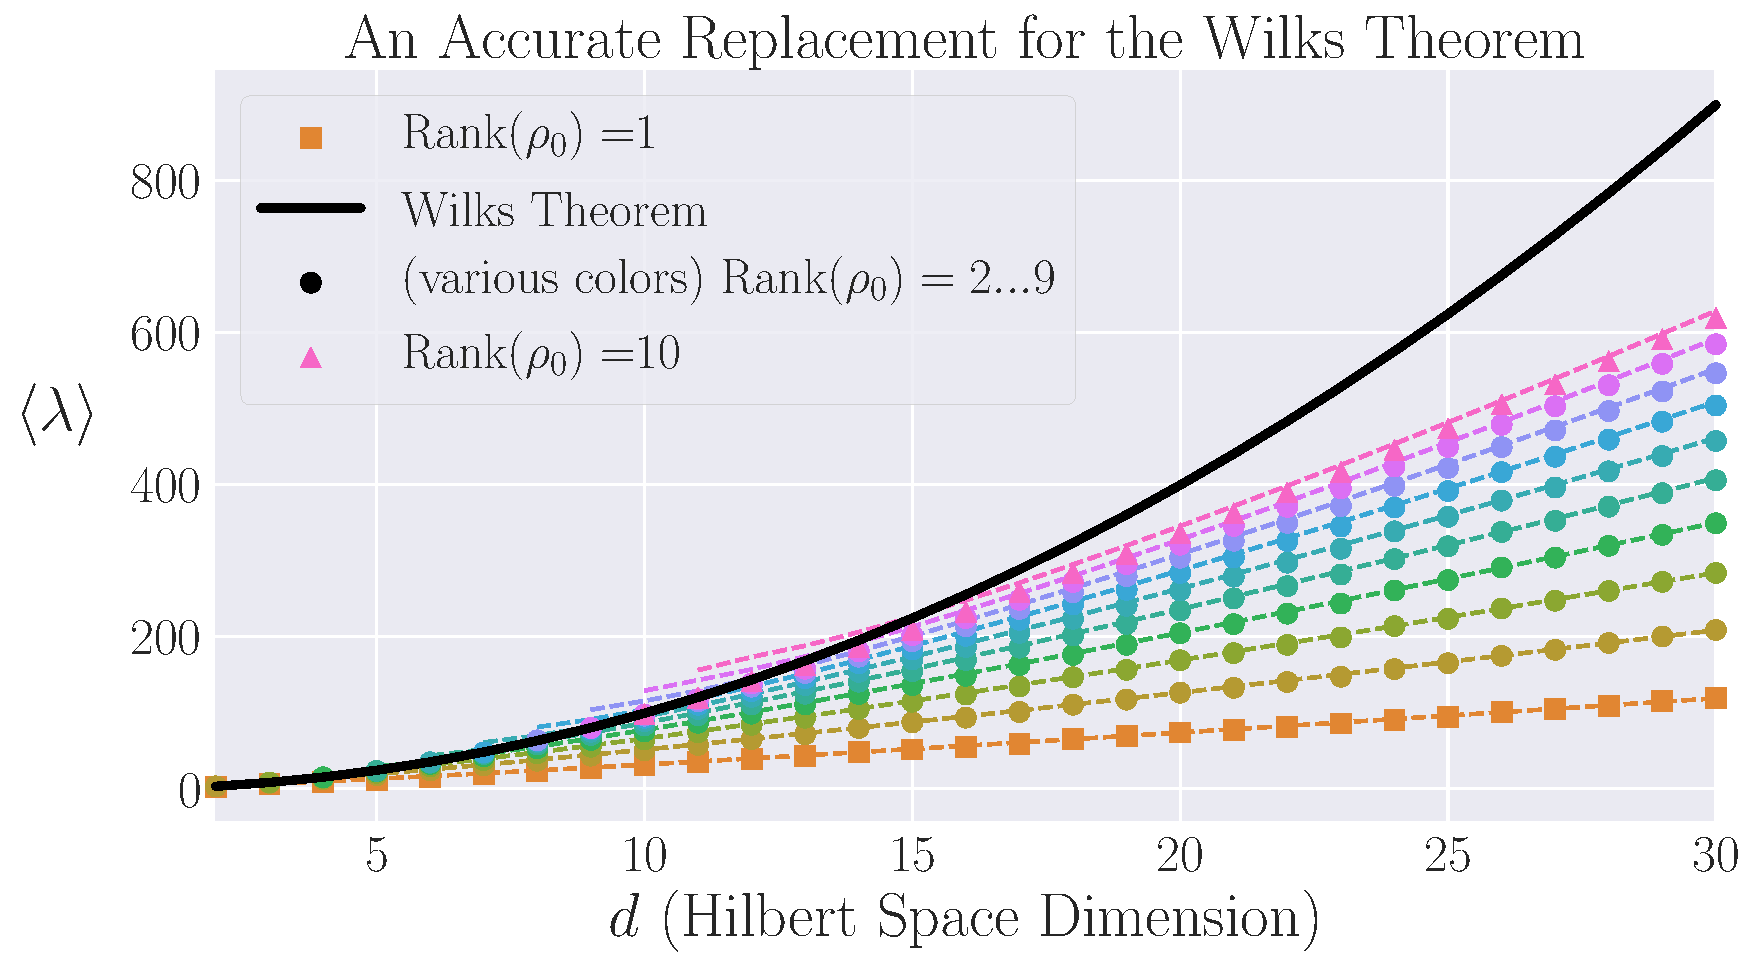
\includegraphics[width=\columnwidth]{Images/Figure_6.pdf}
 \caption{Numerical results for $\expect{\lambda}$ compared to the prediction of the Wilks theorem (solid line) and our replacement theory as given in Equation \eqref{eq:ourLLRS} (dashed lines).  Our formula depends on the rank $r$ of $\rho_0$ (unlike the Wilks prediction), and is nearly perfect for $r\ll d$.  It becomes less accurate as $r$ approaches $d/2$, and is invalid when $r\approx d$.}
 \label{fig:modelcomp-iso}
\end{figure}




\subsection{Comparison to Heterodyne Tomography}
\label{sec:heterotomo}
In practice, the Fisher information is rarely isotropic.  So we tested our idealized result by applying it to a realistic, challenging, and experimentally relevant problem: quantum heterodyne (equivalent to double homodyne) state tomography \cite{Lvovsky2001a, Bertrand1987, Leonhardt1995, Lvovsky2009} of a single optical mode.  (See Figure \ref{fig:fish_condition} for a plot of the \emph{condition number} -- the ratio of the largest eigenvalue to the smallest -- of the estimated Fisher information. It is clear that $\mathcal{I} \not \propto \Id$.) States of this continuous-variable system are described by density operators on the infinite-dimensional Hilbert space $L^2(\reals)$.  Fitting these infinitely many parameters to finitely much data demands simpler models.

\begin{figure}[h]
  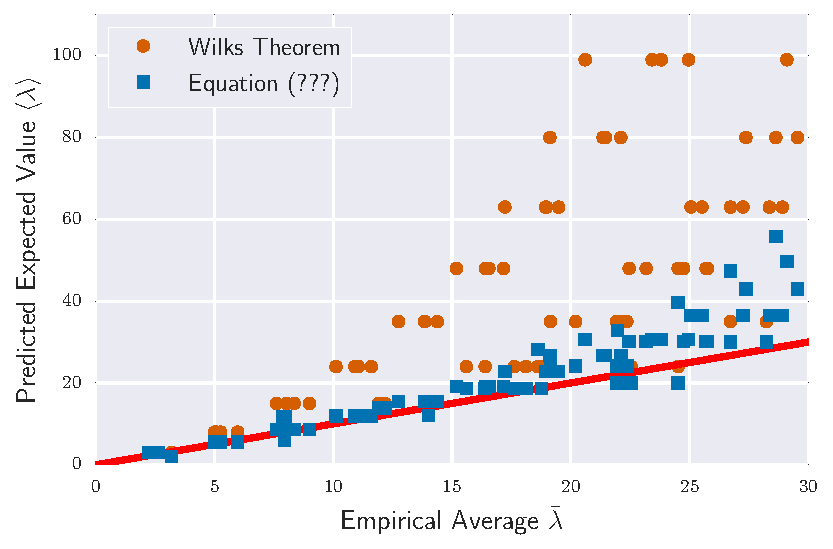
\includegraphics[width=\columnwidth]{Images/Figure_7.pdf}
 \caption{The condition number $\kappa$ -- the ratio of the largest eigenvalue to the smallest -- of the estimated heterodyne Fisher information. (Estimates are the average over 100 Hessians of the loglikelihood function.) $\kappa$ grows with model dimension, meaning anisotropy is increasing.  The dashed lines indicate different states $\rho_{0}$, and the solid line is $\kappa = 1$ (i.e., $\mathcal{I} \propto \Id$.).}
\label{fig:fish_condition}
\end{figure}

We consider a family of nested models motivated by a low-energy (few-photon) ansatz, and choose   
the Hilbert space $\mathcal{H}_d$ to be that spanned by the photon number states $\{\ket{0},\ldots ,\ket{d-1}\}$.
Heterodyne tomography reconstructs $\rho_{0}$ using data from repeated measurements of the 
coherent-state POVM, $\{|\alpha\rangle\langle \alpha| /\pi, ~\alpha=x+ip\in \mathbb{C}\}$, which corresponds to sampling directly from the 
state's Husimi $Q$-function \cite{Husimi1940}.

We examined the behavior of $\lambda$ for 13 distinct states $\rho_{0}$, both pure and mixed, supported on $\mathcal{H}_{2}, \mathcal{H}_{3}, \mathcal{H}
_{4}$, and $\mathcal{H}_{5}$.  We used rejection sampling to simulate 100 heterodyne datasets with up to $N_{\mathrm{samples}}=10^5$, and found MLEs over each of the 9 models $\M_2, \ldots, M_{10}$ using numerical optimization \footnote{The model $\M_{1}$ is trivial, as $\M_{1} = \{|0\rangle \langle 0|\}$. This model will almost always be wrong, in general.}.  For each $\rho_{0}$ and each $d$, we averaged $\lambda(\rho_{0}, \M_{d})$ over all 100 datasets to obtain an empirical average loglikelihood ratio $\bar{\lambda}$ for each $(\rho_0,d)$ pair.

Results of this test are shown in Figure \ref{fig:modelcomp}, where we plot the predictions for $\langle \lambda \rangle$ given by the Wilks theorem and Equation \eqref{eq:ourLLRS}, against the empirical average $\bar\lambda$, for a variety of $\rho_{0}$ and $d$. Our formula correlates very well with the empirical average, while the Wilks theorem (unsurprisingly) overestimates $\lambda$ dramatically for low-rank states.  Whereas a model selection procedure based on the Wilks theorem would tend to falsely reject larger Hilbert spaces (by setting the threshold for acceptance too high), our formula provides a reliable null theory.

\begin{figure}
 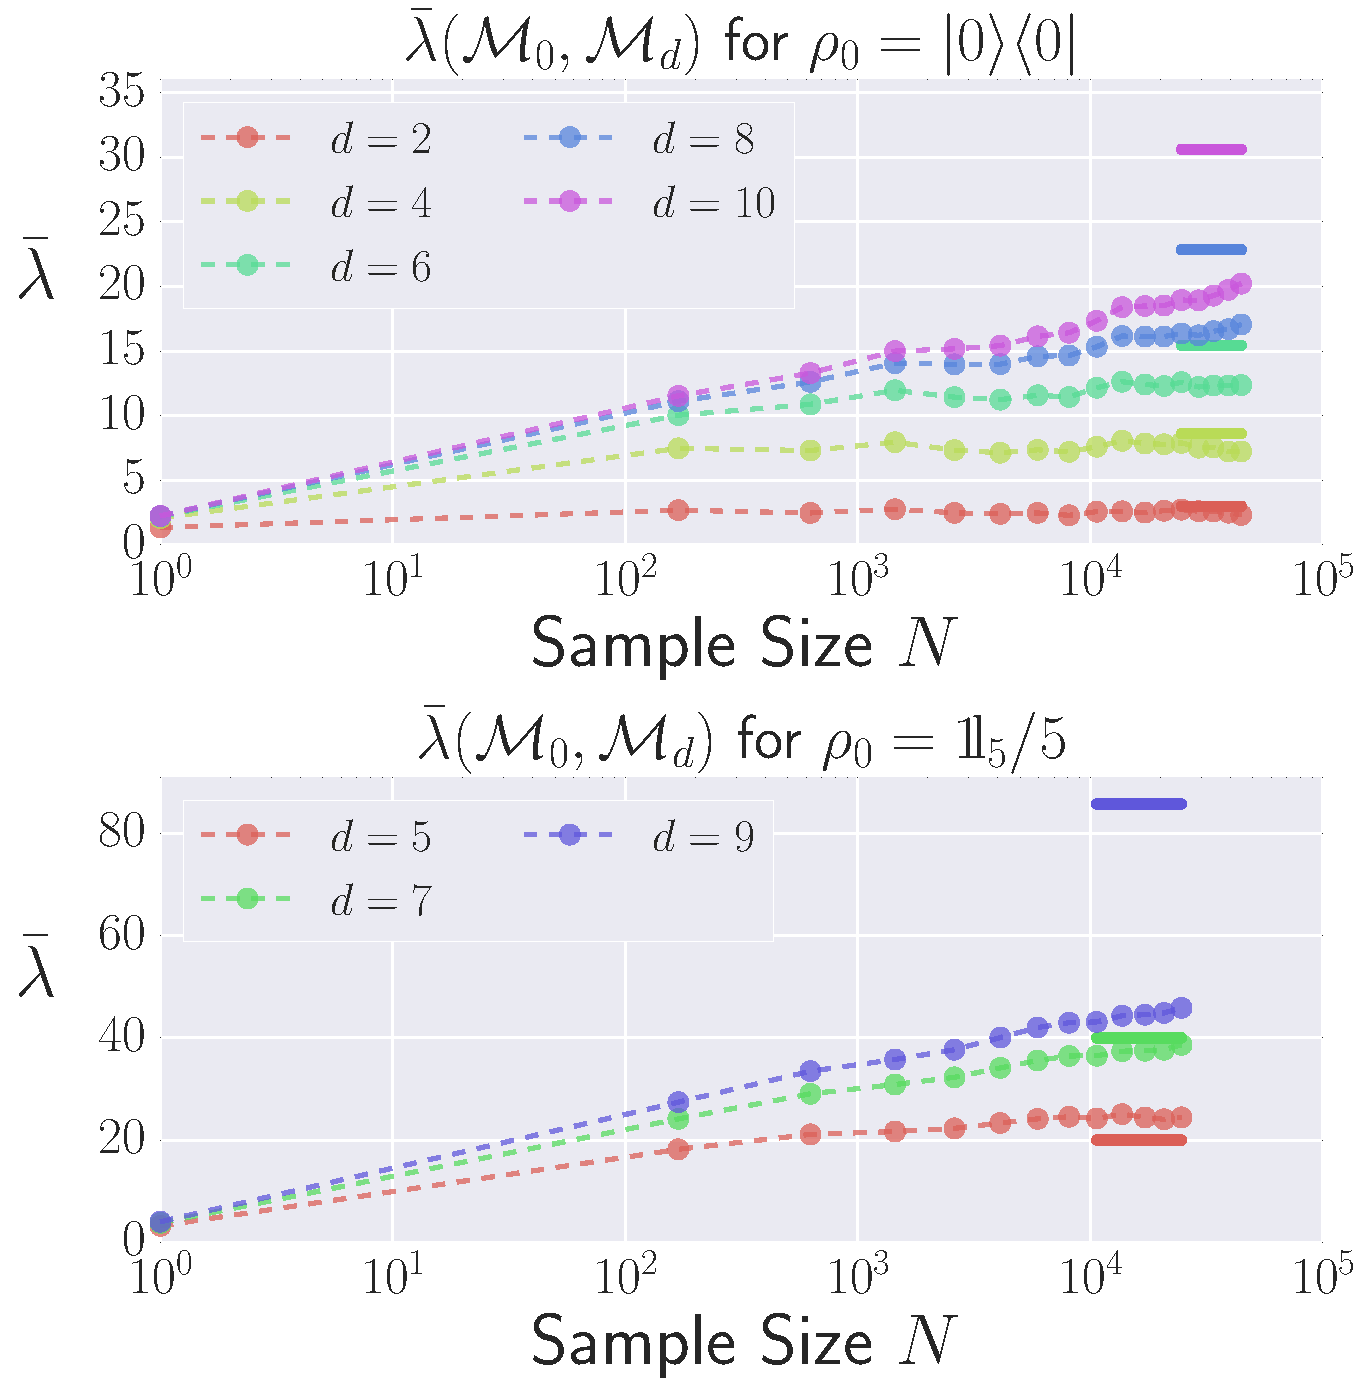
\includegraphics[width=\columnwidth]{Images/Figure_8.pdf}
 \caption{The Wilks theorem (orange dots) dramatically over-estimates $\langle\lambda(\rho_{0}, \M_{d})\rangle$ in optical heterodyne tomography. Our formula, Equation \ref{eq:ourLLRS} (blue squares), is far more accurate. Residual discrepancies occur in large part because $N_{\mathrm{samples}}$ is not yet ``asymptotically large''. The solid red line corresponds to perfect correlation between theory ($\expect{\lambda}$) and practice ($\bar\lambda$).}
 \label{fig:modelcomp}
\todo[inline]{Put the right equation number in here}
\end{figure}

Interestingly, as $d$ grows, Equation \eqref{eq:ourLLRS} also begins to overpredict. As Figure \ref{fig:totalcontrib} indicates, a more accurate description is that the numerical experiments are \emph{underachieving}, because $\bar\lambda$ is still growing with $N_{\mathrm{samples}}$.  Both the Wilks theorem and our analysis are derived in an asymptotic limit $N_{\mathrm{samples}} \rightarrow \infty$; for finite but large $N_{\mathrm{samples}}$, both may be invalid.  Figure \ref{fig:totalcontrib} shows that, even at $N\sim 10^{5}$, the behavior of $\bar{\lambda}$ has failed to become asymptotic. This is surprising, and suggests heterodyne tomography is a particularly exceptional and challenging case to model statistically. 

\begin{figure}
  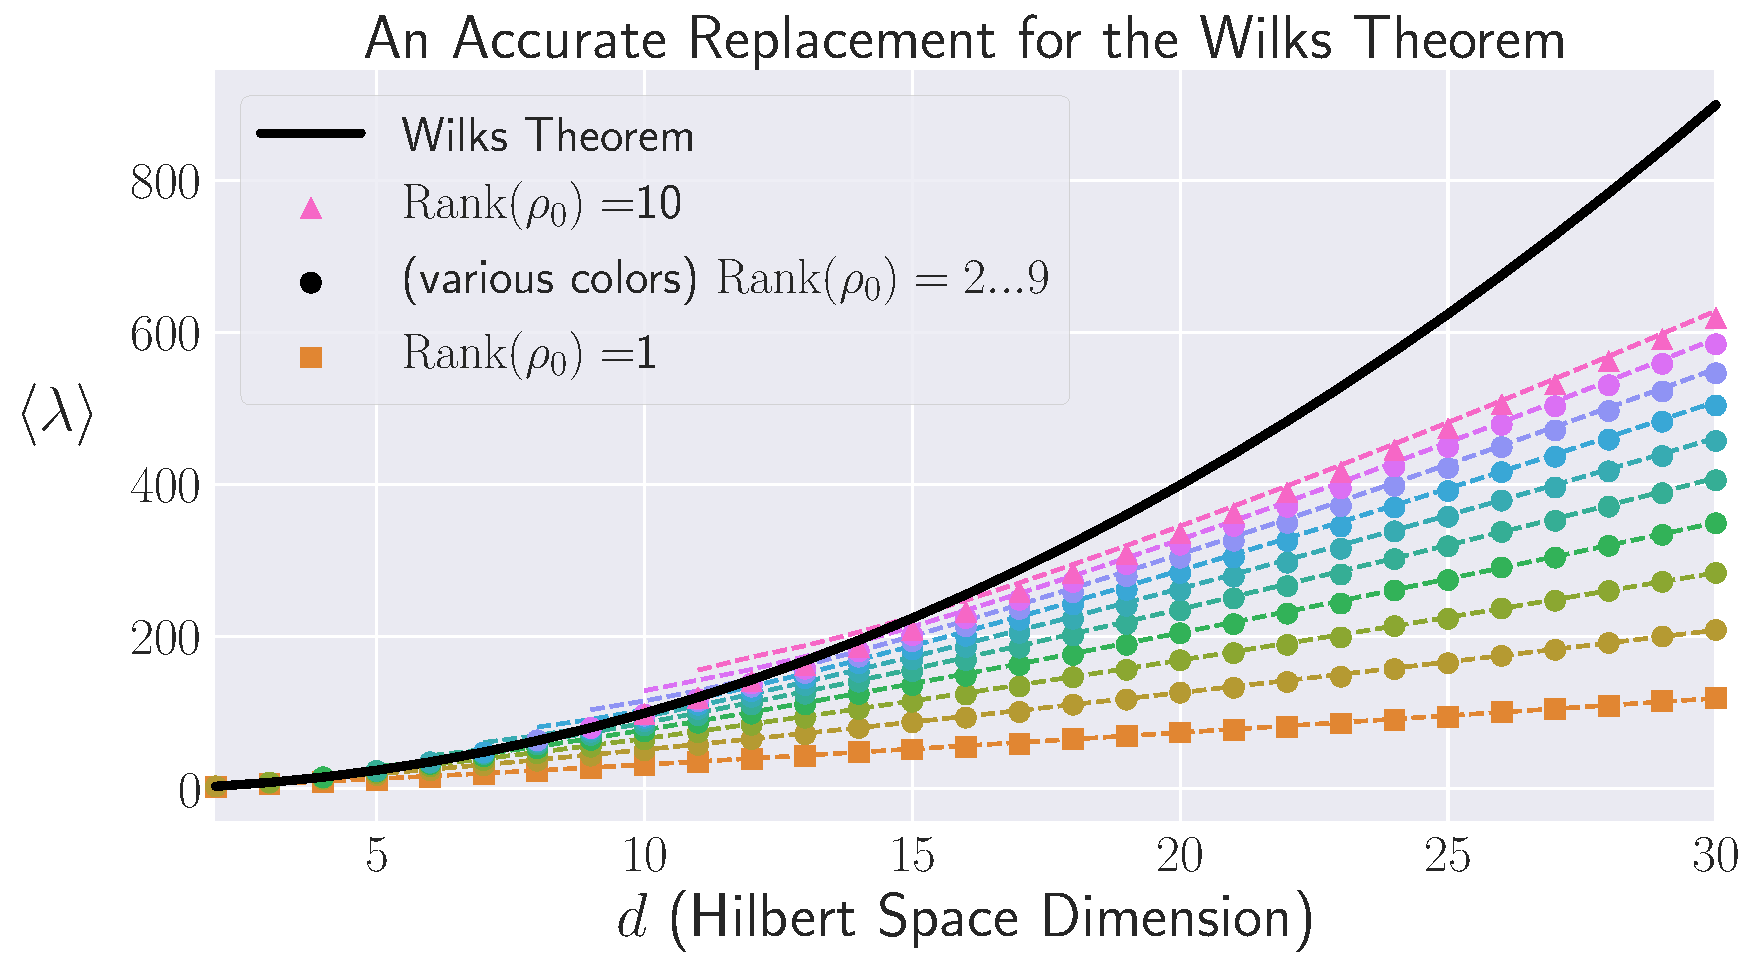
\includegraphics[width=\columnwidth]{Images/Figure_9.pdf}
 \caption{The empirical average $\bar{\lambda}$  may have achieved its asymptotic value, or is still 
growing, depending on the true state $\rho_{0}$ and the model dimension $d$. Solid lines indicate the value of our formula
for the asymptotic expected value, given in Equation \eqref{eq:ourLLRS}.}
\label{fig:totalcontrib}
\end{figure}


However, our model \emph{does} get some of the qualitative features correct. In Figure \ref{fig:model_comparison}, we look at $\langle \lambda_{jk}\rangle$, for an isotropic Fisher information, and for simulated heterodyne tomography. While the values of $\langle \lambda_{jk} \rangle$ do not agree exactly, they still break down into two groups, the ``L" and the ``kite". (See Figure \ref{fig:individcontrib} for an analysis of the discrepancies.)
 
 
\begin{figure}
  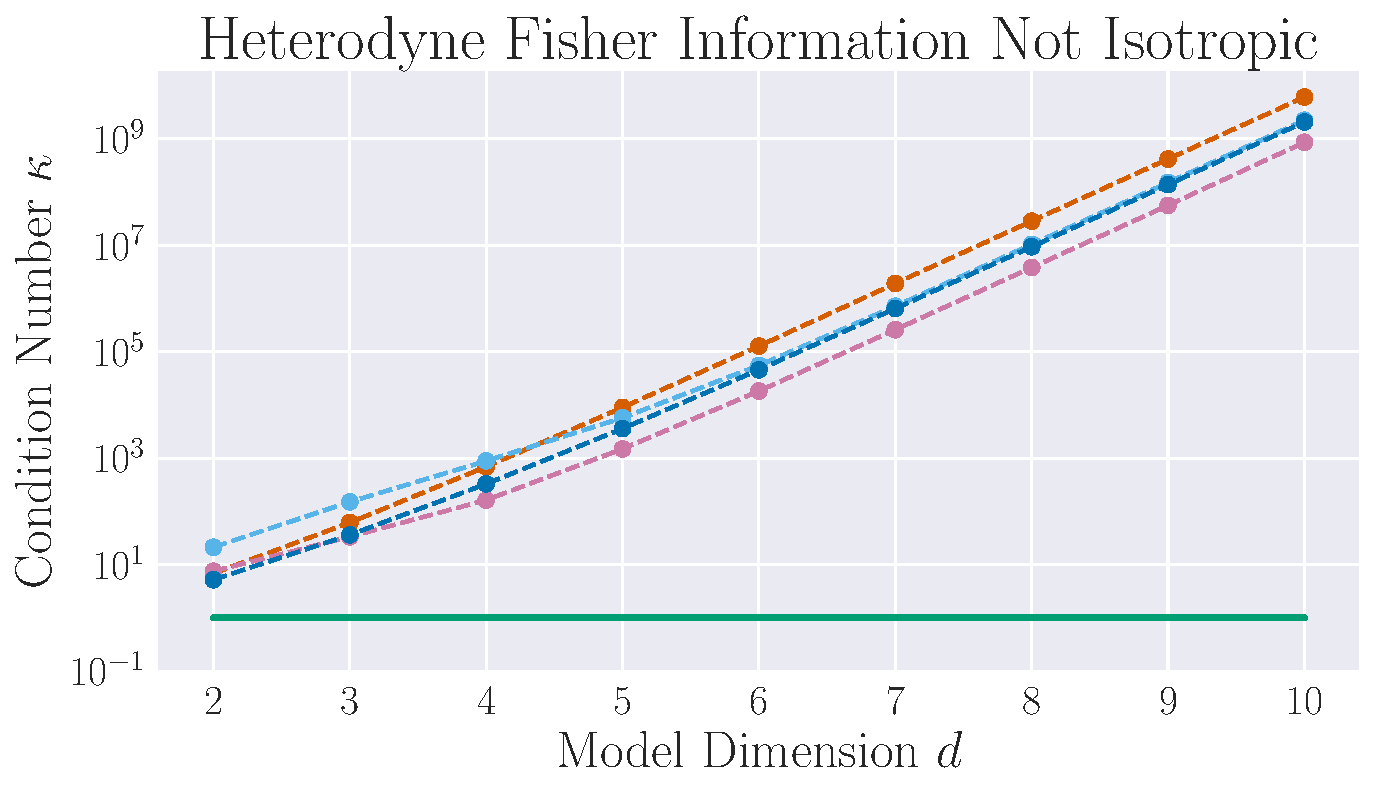
\includegraphics[width=\columnwidth]{Images/Figure_10.pdf}
 \caption{The values of $\langle \lambda_{jk} \rangle$ for an isotropic Fisher information (left), and for heterodyne tomography (right). \textbf{Top}: $\rho_{0} = |0\rangle\langle 0|$. \textbf{Bottom}: $\rho_{0} = \mathcal{I}_{2}/2$. \textbf{Discussion}: Qualitatively, the behavior is the same, though there are quantitative differences, particularly within the kite.}
\label{fig:model_comparison}
\end{figure}

\begin{figure}[h]
  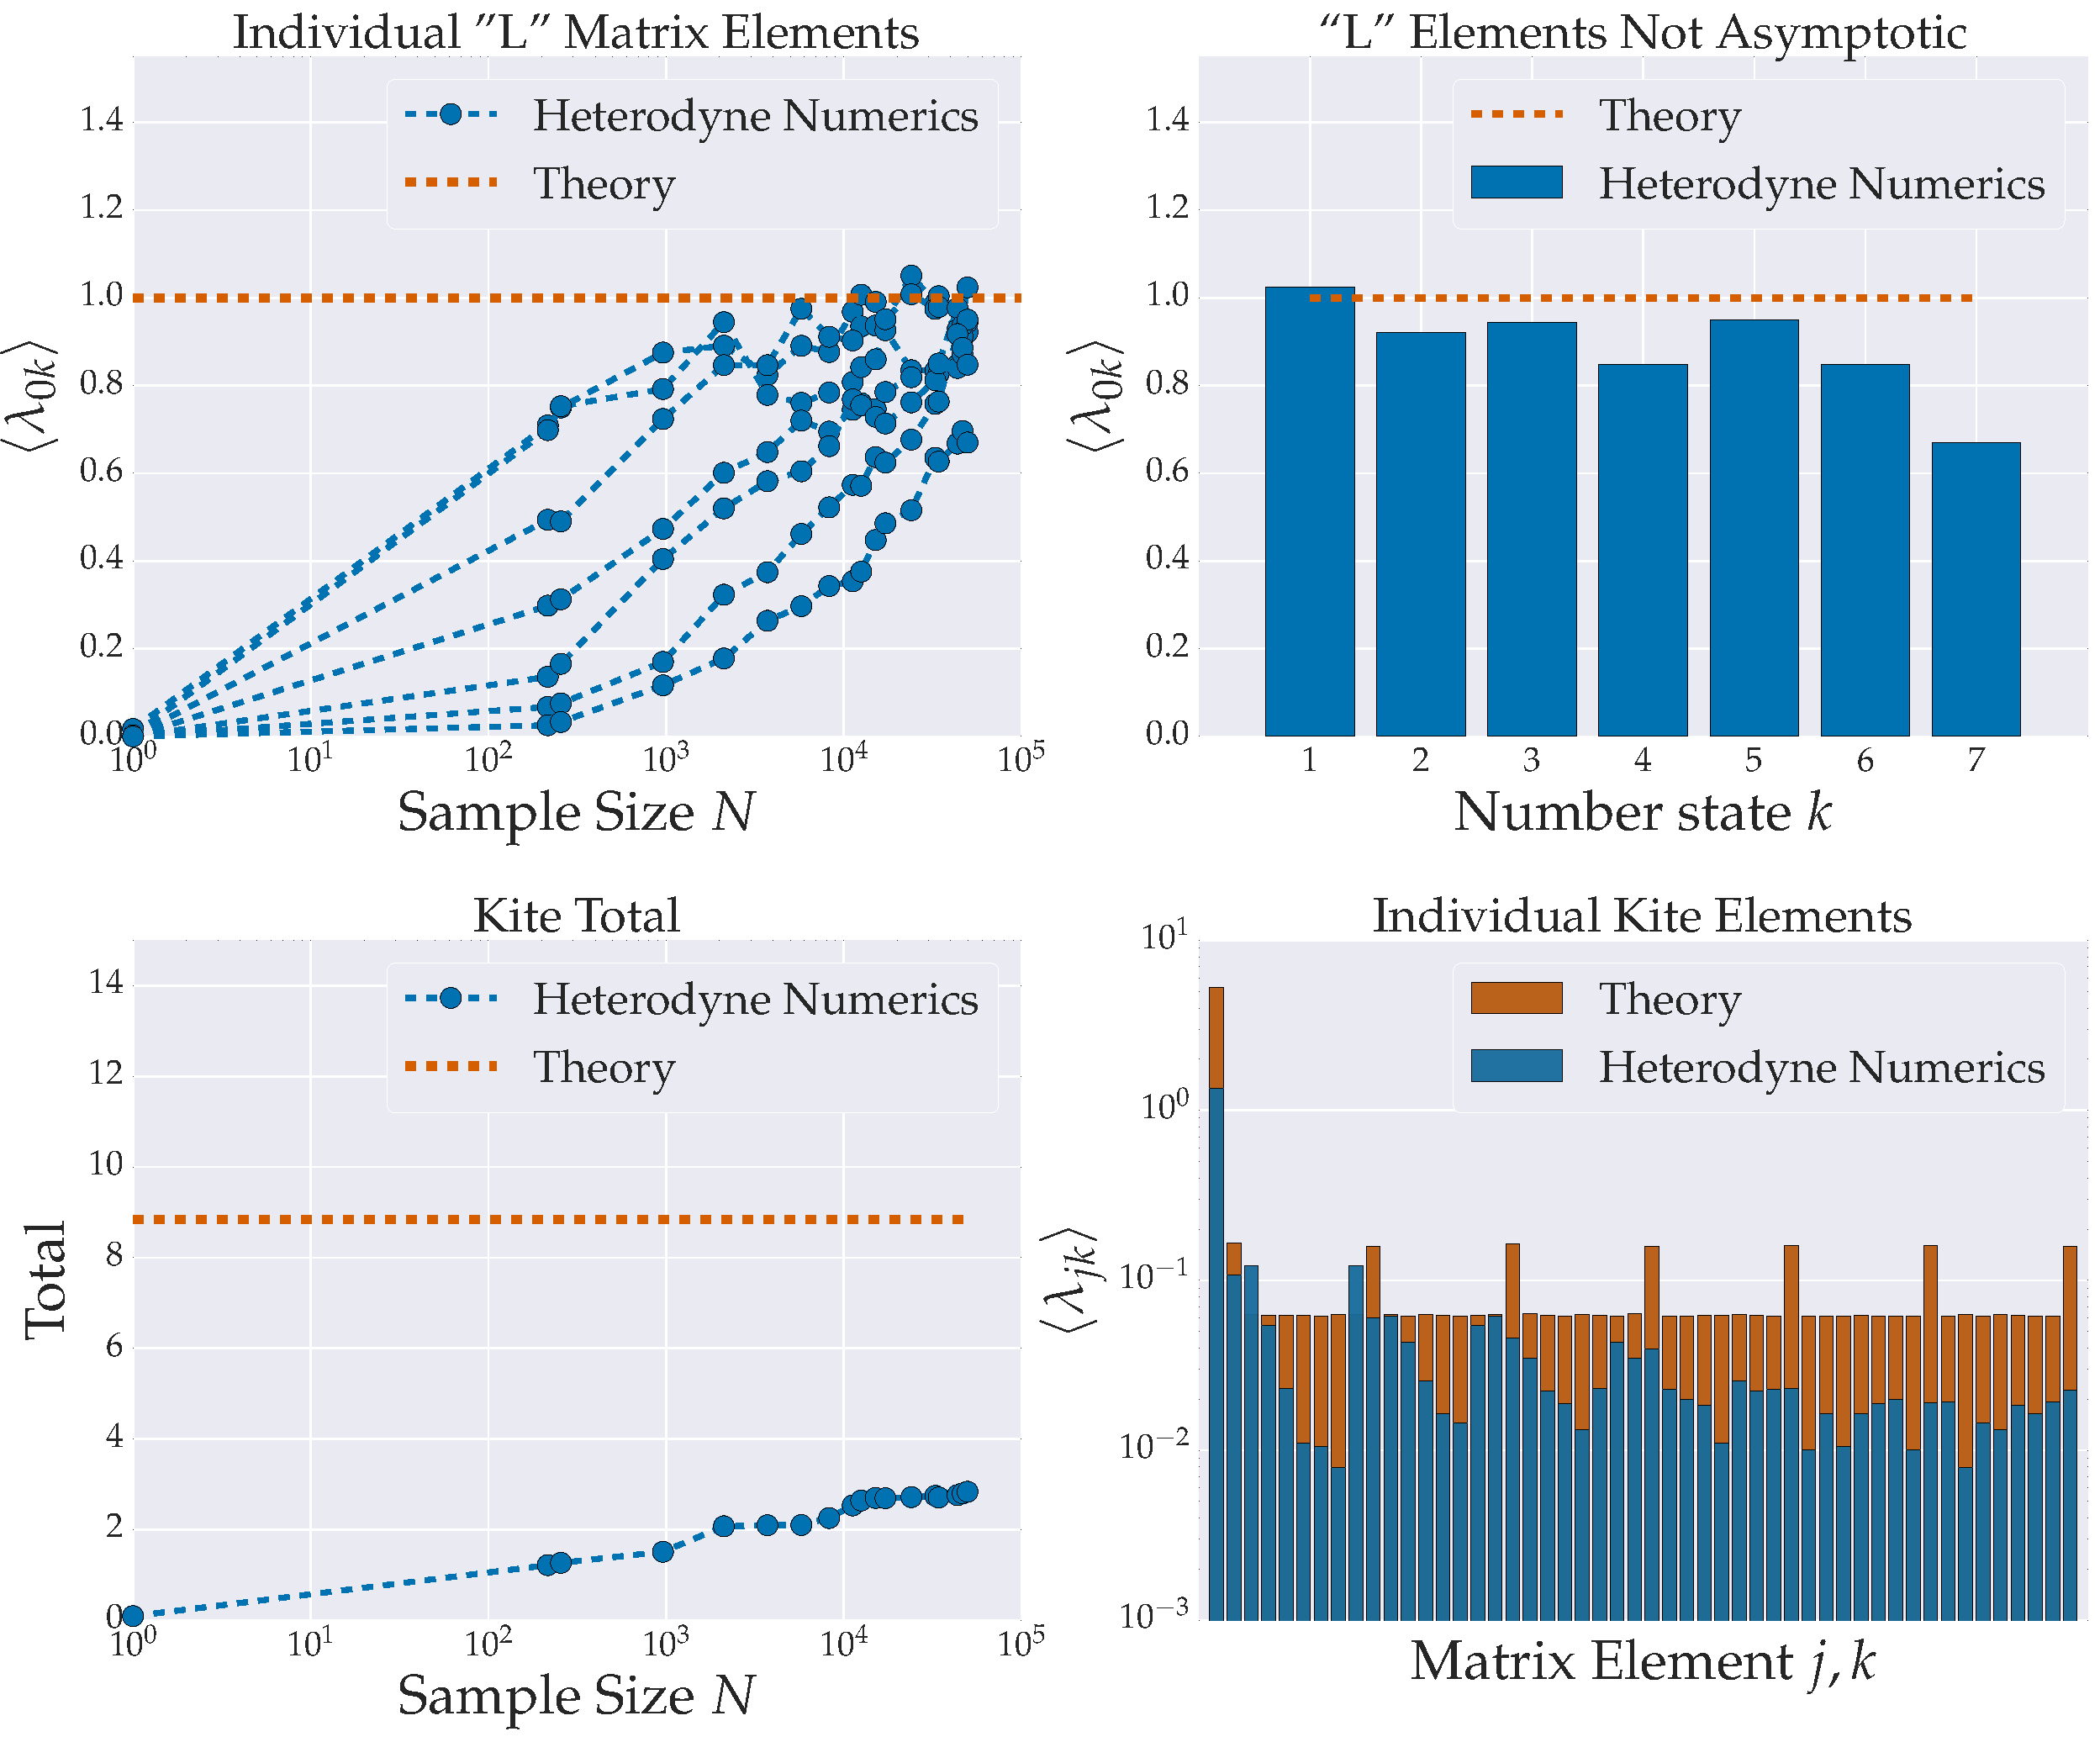
\includegraphics[width=\columnwidth]{Images/Figure_11.pdf}
 \caption{Examining how our predicted values for $\langle \lambda_{jk} \rangle$ disagree with simulated heterodyne experiments. We take $\rho_{0} = |0\rangle\langle 0|$ and $d=8$. \textbf{Top Left}: The values of  $\langle \lambda_{0k}\rangle$ in the ``L" as a function of $N_{\mathrm{samples}}$.  \textbf{Top Right}:  Even at the largest $N_{\mathrm{samples}}$ studied, $\langle \lambda_{0k}\rangle$ is nontrivially less than 1, especially for the higher number states. \textbf{Bottom Left}: The total from the ``kite" versus $N_{\mathrm{samples}}$. It is clear the total is still growing. \textbf{Bottom Right}: The individual ``kite" elements $\langle \lambda_{jk}\rangle$ at the largest $N_{\mathrm{samples}}$ studied;  most are small compared to values they would have in the isotropic case.}
\label{fig:individcontrib}
\end{figure}



\section{Conclusions and Discussion}
The Wilks theorem is not generally reliable in quantum state tomography, but our Equation \eqref{eq:ourLLRS} provides a much more broadly applicable replacement that can be used in model selection methods.  This includes protocols like the AIC and BIC \cite{Akaike1974, Schwarz1978, Kass1995, Burnham2004} that do not explicitly use the Wilks theorem, but rely on the same assumptions (local asymptotic normality, etc).  Null theories of loglikelihood ratios have many other applications, including hypothesis testing \cite{Blume-Kohout2010,Moroder2013} and confidence regions \cite{Glancy2012a}, and our result is directly applicable to them.  Refs. \cite{Moroder2013,Glancy2012a} both point out explicitly that their methods are unreliable near boundaries and therefore cannot be applied to rank-deficient states; our result fixes this outstanding problem.

However, our numerical experiments with heterodyne tomography show unexpected behavior, indicating that quantum tomography can still surprise, and may violate \emph{all} asymptotic statistics results.  In such cases, bootstrapping \cite{Efron1979, Higgins2004} may be the only reliable way to construct null theories for $\lambda$. 

Finally, the \emph{methods} presented here have application beyond the analysis of loglikelihoods.  They shed light on the behavior of $\rhoML{d}$ for rank-deficient states, and can be used to predict other derived properties such as the average rank of the estimate, which is independently interesting for (e.g.) quantum compressed sensing \cite{Flammia2012a, Steffens2016, Kalev2015, Kalev2015a}.

\section{Acknowledgements:} The authors are grateful for those who provide support for the following software packages: iPython/Jupyter \cite{Perez}, matplotlib
\cite{Hunter2007}, mpi4py \cite{Dalcin2011},  NumPy \cite{VanDerWalt2011}, pandas \cite{mckinney2010}, Python 2.7 
\cite{vanRossum}, seaborn \cite{Waskom2016}, and SciPy \cite{Oliphant2007a}. TLS thanks Jonathan A Gross for helpful 
discussions on software design, coding, and statistics, John King Gamble for useful insights on parallelized 
computation and feedback on earlier drafts of this paper, and Daniel Suess, as well as Anupam Mitra, for proofreading edits.

Sandia National Laboratories is a multi-mission laboratory managed and operated by National Technology and Engineering Solutions of Sandia, LLC., a wholly owned subsidiary of Honeywell International, Inc., for the U.S. Department of Energy's National Nuclear Security Administration under contract DE-NA-0003525.

\bibliographystyle{apsrev4-1}
\bibliography{wilkspaper}
\end{document}
